%--------------------------------------------------------------------%
%
% Berkas utama templat LaTeX.
%
% author Petra Barus, Peb Ruswono Aryan, Faris Rizki Ekananda
%
%--------------------------------------------------------------------%
%
% Berkas ini berisi zip(date,months,p) utama dokumen LaTeX yang akan dibuat.
%
%--------------------------------------------------------------------%

\documentclass[bahasa, 12pt, a4paper, onecolumn, oneside, final]{report}

%-------------------------------------------------------------------%
%
% Konfigurasi dokumen LaTeX untuk laporan tesis IF ITB
%
% @author Petra Novandi
%
%-------------------------------------------------------------------%
%
% Berkas asli berasal dari Steven Lolong
%
%-------------------------------------------------------------------%

% Ukuran kertas
\special{papersize=210mm,297mm}

% Setting margin
\usepackage[top=3cm,bottom=3cm,left=4cm,right=3cm]{geometry}

\usepackage{mathptmx}

% Judul bahasa Indonesia
\usepackage[bahasa]{babel}

% Format citation
\usepackage[style=apa,backend=biber]{biblatex}

\usepackage[utf8]{inputenc}
\usepackage{graphicx}
\usepackage{titling}
\usepackage{blindtext}
\usepackage{sectsty}
\usepackage{chngcntr}
\usepackage{etoolbox}
\usepackage[hidelinks]{hyperref}       % Package untuk link di daftar isi. Ubah jadi \usepackage[hidelinks]{hyperref} apabila ingin menghilangkan kotak merah disekitar link
\usepackage{titlesec}       % Package Format judul
\usepackage{titletoc}       % Package Format judul di toc
\usepackage{tocbibind}      % Package untuk masukkan toc, lot, lof ke Daftar Isi
\usepackage{scrwfile}       % Package untuk membuat Daftar Lampiran dari toc
\usepackage{parskip}
\usepackage{afterpage}
\usepackage{relsize}

\graphicspath{{resources/}}   % letak direktori penyimpanan gambar

% Setting daftar lampiran
\newcommand*{\lopname}{DAFTAR LAMPIRAN}
\TOCclone[\lopname]{toc}{atoc}
\addtocontents{atoc}{\protect\value{tocdepth}=-1}
\newcommand\listofappendices{
  \cleardoublepage
  \phantomsection
  \listofatoc
  \addcontentsline{toc}{chapter}{\lopname}
}

\newcommand*\savedtocdepth{}
\AtBeginDocument{%
  \edef\savedtocdepth{\the\value{tocdepth}}%
}

\let\originalappendix\appendix
\renewcommand\appendix{%
  \originalappendix
  \cleardoublepage
  \addtocontents{toc}{\protect\value{tocdepth}=-1}%
  \addtocontents{atoc}{\protect\value{tocdepth}=\savedtocdepth}%

  \titlecontents{chapter}
    [0pt]
    {\bfseries}
    {Lampiran \thecontentslabel.\quad}
    {}
    {\textmd{\dotfill}\contentspage}

  \titleformat{\chapter}[block]
    {\bfseries}
    {\chaptertitlename\ \thechapter.\quad}{0pt}
    {\bfseries}
}

% Hilangkan titik pada toc
% \makeatletter
% \renewcommand{\@dotsep}{10000} 
% \makeatother
\makeatletter
\renewcommand*\@dotsep{1.7}
\makeatother

% Setel title pada chapter-chapter di toc, lof, lot
\titlecontents{chapter}
  [0pt]
  {\bfseries}
  {\MakeUppercase{Bab} \thecontentslabel\quad\uppercase}
  {}
  {\textmd{\dotfill}\contentspage}
\titlecontents{figure}
  [0pt]
  {}
  {Gambar \thecontentslabel.\quad}
  {}
  {\hfill\contentspage}
\titlecontents{table}
  [0pt]
  {}
  {Tabel \thecontentslabel.\quad}
  {}
  {\hfill\contentspage}

% Masukin Daftar Pustaka ke toc
\let\originalprintbibliography\printbibliography
\renewcommand\printbibliography{%
  \phantomsection
  \cleardoublepage
  \originalprintbibliography
  \addcontentsline{toc}{chapter}{\bibname}
}

% Line satu setengah spasi
\renewcommand{\baselinestretch}{1.5}

% Setting judul
\chapterfont{\centering \Large}
\titleformat{\chapter}[display]
  {\Large\centering\bfseries}
  {\chaptertitlename\ \thechapter}{0pt}
    {\Large\bfseries\uppercase}

% Setting nomor pada subbsubsubbab
\setcounter{secnumdepth}{3}

\makeatletter

\makeatother

% Counter untuk figure dan table.
\counterwithin{figure}{section}
\counterwithin{table}{section}

% Define blank page
\newcommand*{\blankpage}{\afterpage{\null\newpage}}

\makeatletter

\makeatother

\addbibresource{references.bib}

\begin{document}

%Basic configuration
\title{PENERAPAN TEORI PERMAINAN DALAM MANAJEMEN WAKTU DAN HUBUNGAN INTERPERSONAL MELALUI PERMAINAN PERSONA 4 GOLDEN}
\date{}
\author{\uppercase{
        Chrysanty Gwyneth Winata Ang \\
        NIM: 10119075 \\}
    (Program Studi Sarjana Matematika) \\
}

\pagenumbering{roman}
\setcounter{page}{1}

\clearpage
\pagestyle{empty}

\begin{center}
    \smallskip

    \large \bfseries \MakeUppercase{\thetitle}
    \vfill

    \large TUGAS AKHIR \\
    \small Karya tulis sebagai salah satu syarat \\
    \small untuk memperoleh gelar sarjana dari \\
    \small Institut Teknologi Bandung
    \vfill

    \large Oleh

    \large \theauthor

    \vfill
    \begin{figure}[h]
        \centering
        
\includegraphics[width=0.15\textwidth]{cover-ganesha.jpg}
    \end{figure}
    \vfill

    \large
    \uppercase{
        Institut Teknologi Bandung \\
        2023 \\
    }
\end{center}

%     \large
%     \uppercase{
%         Program Studi Matematika \\
%         Fakultas Matematika \& Ilmu Pengetahuan Alam \\
%         Institut Teknologi Bandung
%     }

%     November 2022

% \end{center}

\clearpage


\pagestyle{plain}

\clearpage
\chapter*{ABSTRAK}
\addcontentsline{toc}{chapter}{Abstrak}

%taruh abstrak bahasa indonesia di sini
\blindtext
\clearpage
\clearpage
\chapter*{Abstract}
%\addcontentsline{toc}{chapter}{Abstract}

Game theory is the study of mathematical model for cooperation among decision agents. One of the application of game theory is time management and interpersonal relationship. Components of decision problems are action, payoff, preferences, and nature. The result of the aforementioned components are manifested in a payoff function used for subsequent decision.

Game theory could be divided into several types based on the form and completeness of information. Completeness of information divides game theory into complete information and incomplete information. Form of information divides game theory into static and dynamic games. Dynamic games are represented as extensive game form and are said to be a complete information game if there are no nature component. The game Persona 4 Golden is a kind of complete imperfect game, also known as multistage game.

Persona 4 Golden is a role playing game in which the player needs to manage time. The time management done in this game will affect interpersonal relationship with other characters in the game and will also affect the ending of the game's story. Therefore, this final project will explore how to model the decision making, specifically in the game Persona 4 Golden. This final project will also examine various factors which will affect decision making in Persona 4 Golden.

\textit{Keywords:} game theory, time management, interpersonal relationship, Persona 4 Golden
\clearpage
\pagestyle{empty}

\begin{center}
    \smallskip

    \large \bfseries \MakeUppercase{\thetitle}
    \vfill

    \normalfont Oleh

    \normalfont \textbf{Chrysanty Gwyneth Winata Ang} \\

    \normalfont \textbf{NIM: 10119075} \\
    \vspace{0.75cm}

    \normalfont \textbf{Program Studi Sarjana Matematika} \\
    \normalfont \textbf{Institut Teknologi Bandung}

    \vfill

    \normalfont Menyetujui \\
    \vspace{0.75cm}

    \normalfont Pembimbing \\
    \vspace{0.75cm}

    Bandung, 14 Juli 2023 \\

    \vfill
    \rule{7cm}{0.15mm}\\
    (Dr. Aditya Purwa Santika, S.Si., M.Si.)

\end{center}
\clearpage

\chapter*{Kata Pengantar}
\addcontentsline{toc}{chapter}{KATA PENGANTAR}

Puji syukur penulis panjatkan ke hadirat Tuhan Yang Maha Esa, yang telah memberikan rahmat, karunia, dan petunjuk-Nya sehingga penulis dapat menyelesaikan tugas akhir yang berjudul "Penerapan Teori Permainan dalam Manajemen Waktu dan Hubungan Interpersonal Melalui Permainan Persona 4 Golden". Tugas akhir ini merupakan salah satu syarat penulis untuk memperoleh gelar Sarjana Matematika dari Institut Teknologi Bandung.

Tugas akhir ini tidak akan selesai tanpa pihak-pihak yang terlibat. Sehingga, penulis secara khusus mengucapkan terima kasih kepada Bapak Dr. Aditya Purwa Santika, S.Si., M.Si. selaku dosen pembimbing penulis yang telah mendedikasikan waktu dalam membimbing penulisan tugas akhir ini, memberikan banyak masukan berharga, serta memperkenalkan penulis pada permainan \textit{board game}. Penulis juga mengucapkan terima kasih sebesar-besarnya kepada:
\begin{enumerate}
    \item Bapak Dr. Suhadi Wido Saputro, S.Si., M.Si. dan Dr. Agus Yodi Gunawan, S.Si., M.Si. selaku dosen penguji seminar yang telah memberikan pertanyaan dan masukan untuk mengembangkan tugas akhir penulis.
    \item Ibu Dr. Dellavitha, S.Si., M.Si. selaku dosen wali akademik yang telah membantu penulis selama menempuh pendidikan di Institut Teknologi Bandung.
    \item Orang tua penulis, Teja Winata dan Herny Meishintya, dan saudara penulis, Chrystalia Glenys Winata Ang dan Chrystina Giselle Winata Ang yang selalu mendoakan dan memberi dukungan terbaik agar penulis diberi kelancaran selama menempuh pendidikan.
    \item Teman-teman jurusan Matematika dan Aktuaria yang menjadi teman belajar dan teman berjuang selama menyelesaikan pendidikan di jurusan.
    \item Teman-teman kelompok penulis: yee, KSEP ITB, DKV, Sarjana PDP, KMK ITB, Purist MA LOL dan, UKJ ITB yang telah memberikan dukungan moral dan mewarnai kehidupan penulis selama berkuliah.
\end{enumerate}

Semoga tugas akhir ini bermanfaat dan memberikan wawasan bagi pembaca.

\hfill{Bandung, Juli 2023}

\hfill{Penulis}
% \chapter*{Lembar Pernyataan}

Dengan ini saya menyatakan bahwa:

\begin{enumerate}

    \item Pengerjaan dan penulisan Laporan Tugas Akhir ini dilakukan tanpa menggunakan bantuan yang tidak dibenarkan.
    \item Segala bentuk kutipan dan acuan terhadap tulisan orang lain yang digunakan di dalam penyusunan laporan tugas akhir ini telah dituliskan dengan baik dan benar.
    \item Laporan Tugas Akhir ini belum pernah diajukan pada program pendidikan di perguruan tinggi mana pun.

\end{enumerate}

Jika terbukti melanggar hal-hal di atas, saya bersedia dikenakan sanksi sesuai dengan Peraturan Akademik dan Kemahasiswaan Institut Teknologi Bandung bagian Penegakan Norma Akademik dan Kemahasiswaan khususnya Pasal 2.1 dan Pasal 2.2.
\vspace{15mm}

Bandung, 6 Juli 2015 \\
Petra Novandi \\
NIM 13505059


\titleformat*{\section}{\centering\bfseries\Large\MakeUpperCase}
\titlespacing*{\chapter}{0pt}{0pt}{3pc}

% Setting judul toc, lot, lof, bib
\renewcommand{\contentsname}{DAFTAR ISI}
\renewcommand{\listfigurename}{DAFTAR GAMBAR}
\renewcommand{\listtablename}{DAFTAR TABEL}
\renewcommand{\bibname}{DAFTAR PUSTAKA}

\tableofcontents
\listofappendices
\listoffigures
\listoftables

\newpage

\titleformat*{\section}{\bfseries\large}
\pagenumbering{arabic}

%----------------------------------------------------------------%
% Konfigurasi Bab
%----------------------------------------------------------------%
\setcounter{page}{1}
\renewcommand{\chaptername}{BAB}
\renewcommand{\thechapter}{\Roman{chapter}}
%----------------------------------------------------------------%

%----------------------------------------------------------------%
% Dafter Bab
% Untuk menambahkan daftar bab, buat berkas bab misalnya `chapter-6` di direktori `chapters`, dan masukkan ke sini.
%----------------------------------------------------------------%
%\citeall
\nocite{*}
\chapter{Pendahuluan}

\section{Latar Belakang}
\label{sec:latarbelakang}

Di kehidupan sehari-hari, manusia sering kali menghadapi masalah pengambilan keputusan. Pengambilan keputusan tersebut akan berdampak pada keputusan berikutnya, dan akan terus berlanjut hingga mencapai suatu kesimpulan. Manusia sering kali dihadapi dengan berbagai pilihan. Setiap pilihan memiliki konsekuensi minimal berupa waktu yang digunakan ketika mengambil pilihan tersebut. Selain itu, sebagai makhluk sosial manusia sering kali berinteraksi dengan manusia lain. Interaksi yang terjadi sesama manusia sering terjadi karena pilihan yang dilakukan antar manusia.
%Belum ceritain kalo pengambilan terkadang sulit diambil, dan tidak tahu pengambilan keputusan mana yang sebaiknya dipilih karena bingung. Jadi lewat TA ini harapannya bisa membantu agar ketika mengambil keputusan lebih mudah(?)


Dalam ilmu matematika, terdapat teori permainan yang merupakan ilmu yang mempelajari pemodelan matematis dari interaksi strategis antara dua atau lebih pemain dalam suatu permainan. Teori permainan memiliki tiga aspek utama, yaitu: aksi, keluaran, dan preferensi. Tiga aspek ini saling mempengaruhi satu sama lain. Aksi akan mengakibatkan keluaran, keluaran akan menimbulkan pilihan aksi selanjutnya, dan pilihan aksi diurutkan berdasarkan preferensi. Dalam kehidupan nyata, salah satu contoh teori permainan adalah kesetimbangan Nash yang menyatakan bahwa strategi optimal bagi seorang pemain adalah mengikuti strategi awal sambil mengetahui strategi lawan, dan mempertahankan strategi yang sama apabila seluruh pemain lain tidak mengubah strategi.

Permainan peran atau \textit{role-playing game} (RPG) adalah jenis permainan dimana pemain mengambil sebuah peran pada permainan dengan latar belakang fiksi. Pemain bertanggung jawab untuk memerankan suatu peran dan melakukan aksi. Jenis aksi yang dilakukan dapat bermacam-macam, seperti percakapan antar karakter atau melakukan suatu tindakan atau kegiatan. Aksi yang dilakukan merupakan suatu contoh pengambilan keputusan, dimana keputusan yang diambil akan berdampak pada pengembangan karakter selanjutnya. Pengembangan karakter dapat mempengaruhi akhir dari permainan.

Persona 4 Golden (selanjutnya akan disebut juga sebagai P4G) adalah permainan peran dari yang dibuat oleh perusahaan video gim Jepang, Atlus. Permainan P4G pertama kali rilis di PlayStation Vita pada tahun 2012 dan Windows pada tahun 2020. Permainan P4G memiliki latar waktu pada tahun 2011, dimana karakter utama (atau dikenal sebagai Narukami Yuu) harus menyelesaikan misteri kasus pembunuhan berantai yang terjadi di kota Inaba.

Dalam permainan P4G, terdapat dua jenis aksi penting. Yang pertama, ketika karakter utama masuk dalam \textit{dungeon}. Di dalam \textit{dungeon}, karakter utama akan menggunakan berbagai Persona untuk bertarung dan menyelamatkan karakter lain yang terjebak dalam \textit{dungeon} tersebut. Persona adalah atribut yang digunakan karakter ketika masuk ke \textit{dungeon}. Persona akan membantu karakter ketika bertarung dalam \textit{dungeon} melawan \textit{shadows}. Apabila karakter lain gagal diselamatkan, permainan berakhir dan permainan dinyatakan berakhir buruk. Aksi yang dilakukan dalam \textit{dungeon} sangat krusial karena akan berdampak pada epilog permainan ini. Yang kedua, ketika karakter utama bersosialisasi dengan karakter lain. Relasi antara karakter utama dengan karakter lain dinyatakan dalam bentuk \textit{social link}. Semakin erat relasi yang dimiliki antar karakter, maka \textit{social link} akan semakin tinggi. Akibatnya, Persona yang dimiliki akan semakin kuat dan harapannya \textit{dungeon} dapat diselesaikan dengan lebih cepat dan mudah.

Rentang waktu permainan P4G terbatas dari bulan April 2011 hingga Maret 2012. Sehingga, karakter utama harus menstrategikan pemilihan keputusan terbaik yang dilakukan setiap hari dalam permainan.

Tujuan utama dari tugas akhir ini adalah menerapkan teori permainan dalam manajemen waktu dan hubungan interpersonal sehari-hari yang dimodelkan melalui permainan Persona 4 Golden. Sehingga, pada tugas akhir ini akan dimodelkan pemilihan keputusan terbaik untuk memaksimalkan level \textit{social link} seluruh Persona. Model ini akan digunakan untuk memaksimalkan potensi hubungan interpersonal terbaik dan manajemen waktu dalam permainan. Adapun manfaat dari tugas akhir ini adalah untuk untuk mengaplikasikan teori permainan dalam manajemen waktu dan hubungan interpersonal dalam kehidupan sehari-hari agar tercipta potensi pilihan terbaik dalam pengambilan keputusan.

Tugas akhir ini terdiri atas 4 bab dengan sistematika penulisan sebagai berikut.

Pada bab pertama, dijelaskan mengenai latar belakang, tujuan, manfaat, dan sistematika penulisan dari tugas akhir.

Pada bab kedua, dijelaskan mengenai teori permainan sebagai landasan utama tugas akhir. Bagian ini menjelaskan definisi, aksioma, bentuk, dan konsep teori permainan.

Pada bab ketiga, dijelaskan mengenai faktor-faktor yang mempengaruhi hubungan interpersonal, khususnya dalam permainan Persona 4 Golden. Selain itu, dijelaskan pula mengenai simulasi manajemen waktu dalam permainan Persona 4 Golden.

Pada bab keempat, dijelaskan mengenai rangkuman, kesimpulan, dan masalah terbuka dari tugas akhir.
% \section{Rumusan Masalah}
% Dengan waktu yang terbatas, karakter utama harus memaksimalkan \textit{social link} seluruh Persona. \textit{Social link} mempengaruhi keberhasilan penyelesaian permainan dan kemudahan karakter menyelesaikan permainan ketika berada di \textit{dungeon}.

% Penelitian ini menjawab permasalahan pengambilan keputusan, yang secara spesifik dilakukan pada permainan P4G. Sehingga, rumusan masalah dari tugas akhir ini adalah sebagai berikut.
% \begin{enumerate}
%     \item Bagaimana cara mengkonstruksi fungsi \textit{payoff} sehingga pengambilan keputusan dalam permainan P4G optimal?
%     \item Bagaimana algoritma penyelesaian masalah pemilihan keputusan akan diimplementasikan pada permainan P4G?
% \end{enumerate}

% \section{Tujuan}
% Berdasarkan rumusan masalah yang telah ditulis pada subbab berikutnya, tujuan dari tugas akhir ini adalah sebagai berikut.
% \begin{enumerate}
%     \item Melakukan konstruksi fungsi \textit{payoff} untuk pengoptimalan pengambilan keputusan dalam permainan P4G.
%     \item Mengimplementasikan algoritma masalah pengambilan keputusan pada permainan P4G.
% \end{enumerate}

% \section{Batasan Masalah}
% Dalam tugas akhir ini, terdapat asumsi yang digunakan. Sehingga, batasan masalah yang ditetapkan untuk tugas akhir ini adalah sebagai berikut.
% \begin{enumerate}
%     \item Data yang digunakan berasal dari data hasil permainan, sehingga data yang tidak lengkap akan diasumsikan tidak ada atau berada pada suatu titik  atau batasan tertentu.
% \end{enumerate}

% \section{Metodologi}
% Metodologi atau tahapan yang digunakan dalam tugas akhir ini adalah sebagai berikut.
% \begin{enumerate}
%     \item Mempelajari teori permainan dan permainan peran berdasarkan buku atau jurnal ilmiah yang relevan.
%     \item Mengumpulkan data terkait masalah pengambilan keputusan yang akan diuji.
%     \item Membuat algoritma masalah pengambilan keputusan permainan P4G.
%     \item Mengimplementasikan algoritma masalah pengambilan keputusan.
%     \item Melakukan analisis dari hasil implementasi algoritma masalah pengambilan keputusan.
% \end{enumerate}

\newtheorem{definisi}{Definisi}

\chapter{Teori Permainan}
\section{Teori Permainan}
%bahas game theory
Teori permainan yang merupakan ilmu yang mempelajari pemodelan matematis untuk masalah dan kerja sama antara agen pengambil keputusan. Pengambil keputusan yang selanjutnya disebut sebagai pemain umumnya memiliki informasi yang berguna untuk proses pengambilan keputusan selanjutnya. Pemain harus mengetahui tiga hal yang mendasari masalah ini, seperti: Apa saja pilihan yang mungkin dilakukan? Apa saja hasil dari setiap pilihan? Bagaimana efek dari hasil tersebut (Tadelis, 2011)?

Pengamatan sederhana diatas memberikan definisi pertama yang penting untuk setiap masalah pengambilan keputusan.
\begin{definisi}
    \textbf{Masalah pengambilan keputusan} terdiri atas tiga komponen penting:
    \begin{enumerate}
        \item \textbf{Aksi}, yaitu seluruh alternatif pilihan yang dapat dilakukan pemain.
        \item \textbf{Payoff}, yaitu seluruh konsekuensi yang dapat terjadi dari aksi.
        \item \textbf{Preferensi}, yaitu deskripsi bagaimana pemain mengurutkan himpunan keluaran dari yang paling diinginkan hingga paling tidak diinginkan.
    \end{enumerate}
\end{definisi}

\begin{figure}
    \centering
    \tikzstyle{terminal} = [rectangle, rounded corners, draw=black, fill=blue!30, inner sep=.2cm, text width=3.5cm, align=flush center]
\tikzstyle{others} = [rectangle, text centered, draw=black, inner sep=.2cm, align=flush center, text width=2.5cm]
\tikzstyle{arrow} = [draw, thick, ->, >=stealth]

\newcommand{\factorcolor}{red!30}
\newcommand{\externalcolor}{cyan!10}
\newcommand{\payoffcolor}{green!20}

\begin{tikzpicture}[node distance=2cm]
  \matrix[column sep=1cm, row sep=7mm]{
                                                           & \node (pref) [others, fill=\factorcolor] {Preferensi};           &
    \node (nat) [others, fill=\externalcolor] {\textit{Nature}};                                                          \\
    \node (dp) [terminal] {Masalah Pengambilan Keputusan}; &
    \node (act) [others, fill=\factorcolor] {Aksi};        &                                                                    \\
                                                           & \node (po) [others, fill=\factorcolor] {\textit{Payoff}}; &
    \node (fpo) [others, fill=\payoffcolor] {Fungsi \textit{Payoff}};                                                    \\
  };

  \begin{scope}[every path/.style=arrow]
    \path (dp) -- (act);
    \path (dp) |- (pref);
    \path (dp) |- (po);
    \path (po) -- (fpo);
    \path [dashed] (pref) -- (act);
    \path [dashed] (act) -| (fpo);
    \path [dashed] (nat) -- (fpo);
  \end{scope}
\end{tikzpicture}
    \caption{Diagram Alir Masalah Pengambilan Keputusan}
\end{figure}
Relasi preferensi dinyatakan dalam notasi $\succsim$, yang menyatakan relasi antar \textit{payoff} yang dapat menunjukkan preferensi pemain. Sebagai contoh, misalkan terdapat seorang pemain yang ingin memilih rasa es krim vanila atau stroberi. Pilihan rasa es krim ini dapat di lambangkan sebagai himpunan aksi yang akan dipilih pemain yaitu  $A = \lbrace v, s\rbrace$, dimana $v$ menyatakan rasa vanila dan $s$ menyatakan rasa stroberi. Aksi yang dipilih pemain dapat berupa kondisi dimana pemain memutuskan untuk memakan es krim rasa vanila atau stroberi. Hal ini dapat ditulis sebagai himpunan bayaran $P = \lbrace V, S\rbrace$.
% Bab Studi Literatur digunakan untuk mendeskripsikan kajian literatur yang terkait dengan persoalan tugas akhir. Tujuan studi literatur adalah:

% \begin{enumerate}
%     \item menunjukkan kepada pembaca adanya gap seperti pada rumusan masalah yang memang belum terselesaikan,
%     \item memberikan pemahaman yang secukupnya kepada pembaca tentang teori atau pekerjaan terkait yang terkait langsung dengan penyelesaian persoalan, serta
%     \item menyampaikan informasi apa saja yang sudah ditulis/dilaporkan oleh pihak lain (peneliti/Tugas Akhir/Tesis) tentang hasil penelitian/pekerjaan mereka yang sama atau mirip kaitannya dengan persoalan tugas akhir.
% \end{enumerate}


% \section{Contoh Subbab}
% Perujukan literatur dapat dilakukan dengan menambahkan entri baru di berkas. Tulisan ini merujuk pada \parencite{knuth2001art,vasp1} atau \parencite{4026885} dan \parencite{Kim2006}

% Sekarang mau ke bab berapa yaaaa.... hmm... ke bab \ref{sec:latarbelakang} ahhhhh.

% \blindtext

% \subsection{Contoh Subsubbab}

% \blindtext

% \begin{figure}[h]
%     \centering
%     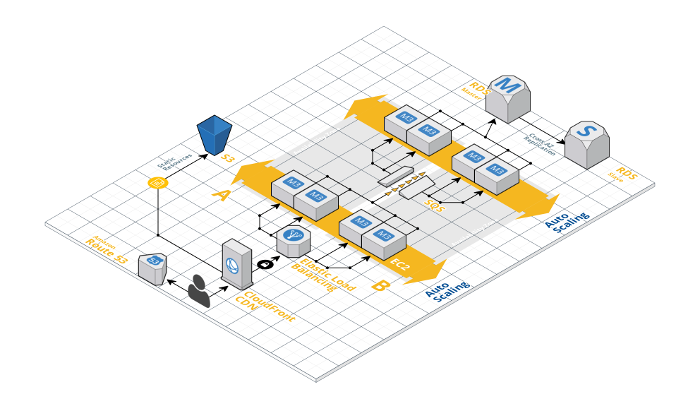
\includegraphics[width=0.8\textwidth]{chapter-2-infrastructure-diagram.png}
%     \caption{Contoh gambar}
% \end{figure}

% \subsubsection{Subsubsubbab}

% \blindtext

% \begin{table}[h]
%     \caption{Tabel random}
%     \vspace{0.25cm}
%     \begin{center}
%         \begin{tabular}{|c|c|c|c|}
%             \hline
%             Title1 & Title2 & Title3 & Title4  \tabularnewline
%             \hline
%             1647   & 1.97   & 0.68   & 1.90 \tabularnewline
%             2301   & 2.92   & 1.06   & 2.75 \tabularnewline
%             2969   & 3.23   & 1.16   & 3.78 \tabularnewline
%             3791   & 4.39   & 1.40   & 4.14 \tabularnewline
%             4625   & 6.72   & 1.87   & 5.59 \tabularnewline
%             \hline
%         \end{tabular}
%     \end{center}
% \end{table}

% \section{Menyisipkan Persamaan}

% Beberapa contoh menyisipkan persamaan.


% \subsection{Contoh Bikin Equation}
% \textbf{text tebal} dan ini \emph{miring}, bikin persamaan di baris yang sama, tinggal pake dolar2 $\Psi(\vec{r}_1,...,\vec{r}_N)$, sehingga persamaan Schr\"{o}dinger, terus, persamaan yang dinomeri kayak gini
% %ini contoh bikin persamaan, ..... :D
% \begin{equation}
%     \left[ \sum_{i}^{N}-\frac{\hbar^2}{2m}\nabla_i^2 + \sum_{i}^{N}V(\vec{r}_i)+ \sum_{i<j}^{N}(\vec{r}_i,\vec{r}_j)\right]\Psi = E\Psi
% \end{equation}

% untuk $N$-elektron, dengan $\hat{H}$=Hamiltonian, $E$=Energi total, $\hat{T}$=Energi kinetik, $\hat{V}$=Energi potensial, dan $\hat{U}$=Interaksi ektron-elektron.

% \subsection{Bikin Matrix}
% Lalalallala.... bikin matrix sekarang, yang ini dikecilin, pake smaller
%     {\smaller
%         \begin{equation}
%             \Psi({\bf r}_1, {\bf r}_2, \cdots {\bf r}_N) = \frac{1}{\sqrt{N!}}\left| \begin{array}{llcl}
%                 \phi_1({\bf r}_1)     & \phi_2({\bf r}_1)     & \cdots                & \phi_N({\bf r}_1)     \\
%                 \phi_1({\bf r}_2)     & \phi_2({\bf r}_2)     & \cdots                & \phi_N({\bf r}_2)     \\
%                 \phi_1({\bf r}_3)     & \phi_2({\bf r}_3)     & \cdots                & \phi_N({\bf r}_3)     \\
%                 \multicolumn{1}{c}{.} & \multicolumn{1}{c}{.} & \multicolumn{1}{c}{.} & \multicolumn{1}{c}{.} \\
%                 \multicolumn{1}{c}{.} & \multicolumn{1}{c}{.} & \multicolumn{1}{c}{.} & \multicolumn{1}{c}{.} \\
%                 \multicolumn{1}{c}{.} & \multicolumn{1}{c}{.} & \multicolumn{1}{c}{.} & \multicolumn{1}{c}{.} \\
%                 \phi_1({\bf r}_N)     & \phi_2({\bf r}_N)     & \cdots                & \phi_N({\bf r}_N)     \\
%             \end{array} \right|
%         \end{equation}
%     }


\chapter{Simulasi Manajemen Waktu dengan Permainan Persona 4 Golden}
Sebagai makhluk sosial, manusia bergantung pada interaksi sosial untuk kelangsungan hidup dan perkembangan pribadi. Interaksi sosial membantu manusia dalam membentuk identitas dan karakter. Manusia sering kali menghadapi masalah pengambilan keputusan ketika melakukan interaksi sosial. Pengambilan keputusan tersebut dapat berdampak pada hubungan interpersonal dengan manusia lain dan juga keputusan yang akan datang. Melalui teori permainan yang diaplikasikan dalam permainan Persona 4 Golden, akan diciptakan model pengambilan keputusan sehingga manusia memiliki potensi pilihan terbaik dan dapat mengambil keputusan terbaik pada suatu kondisi.

Melalui permainan Persona 4 Golden, akan dilakukan pemodelan interaksi sosial yang terjadi dalam permainan, sehingga hubungan interpersonal dengan karakter lain dapat terjalin secara maksimal. Pada bagian selanjutnya akan dijelaskan hubungan sosial dalam permainan Persona 4 Golden, faktor-faktor yang memengaruhi hubungan sosial, dan simulasi pengaturan waktu dalam melakukan interaksi sosial di permainan Persona 4 Golden.

\section{\textit{Social Link}}
%https://www.polygon.com/guides/21284344/persona-4-golden-social-links-guide
\textit{Social link} merepresentasikan hubungan sosial antara karakter utama dengan karakter lainnya. Dalam permainan P4G, terdapat 23 \textit{social link} yang perlu ditingkatkan, dengan rincian:
\begin{enumerate}
    \item 3 \textit{social link} ditingkatkan secara otomatis.
    \item 2 \textit{social link} ditingkatkan dengan menyelesaikan misi.
    \item 1 \textit{social link} ditingkatkan secara manual sebanyak 6 level.
    \item 17 \textit{social link} ditingkatkan secara manual sebanyak 10 level.
\end{enumerate}
%https://www.rpgsite.net/feature/9850-persona-4-golden-social-link-guide-dialogue-options-love-interests-and-full-s-link-walkthroughs
Perhatikan bahwa terdapat hal-hal penting untuk meningkatkan \textit{social link}, yaitu:
\begin{enumerate}
    {\item Setiap \textit{social link} mulai dengan cara yang berbeda. Dalam pembahasan ini, akan dikaji \textit{social link} yang melibatkan pembagian waktu siang dan malam, yaitu:
          \begin{itemize}
              \item 17 \textit{social link} ditingkatkan secara manual sebanyak 10 level.
              \item 1 \textit{social link} ditingkatkan secara manual sebanyak 6 level (karakter Adachi).
              \item 1 \textit{social link} ditingkatkan dengan menyelesaikan misi (karakter Fox).
          \end{itemize}
          }
          \begin{figure}[htbp]
              \centering
              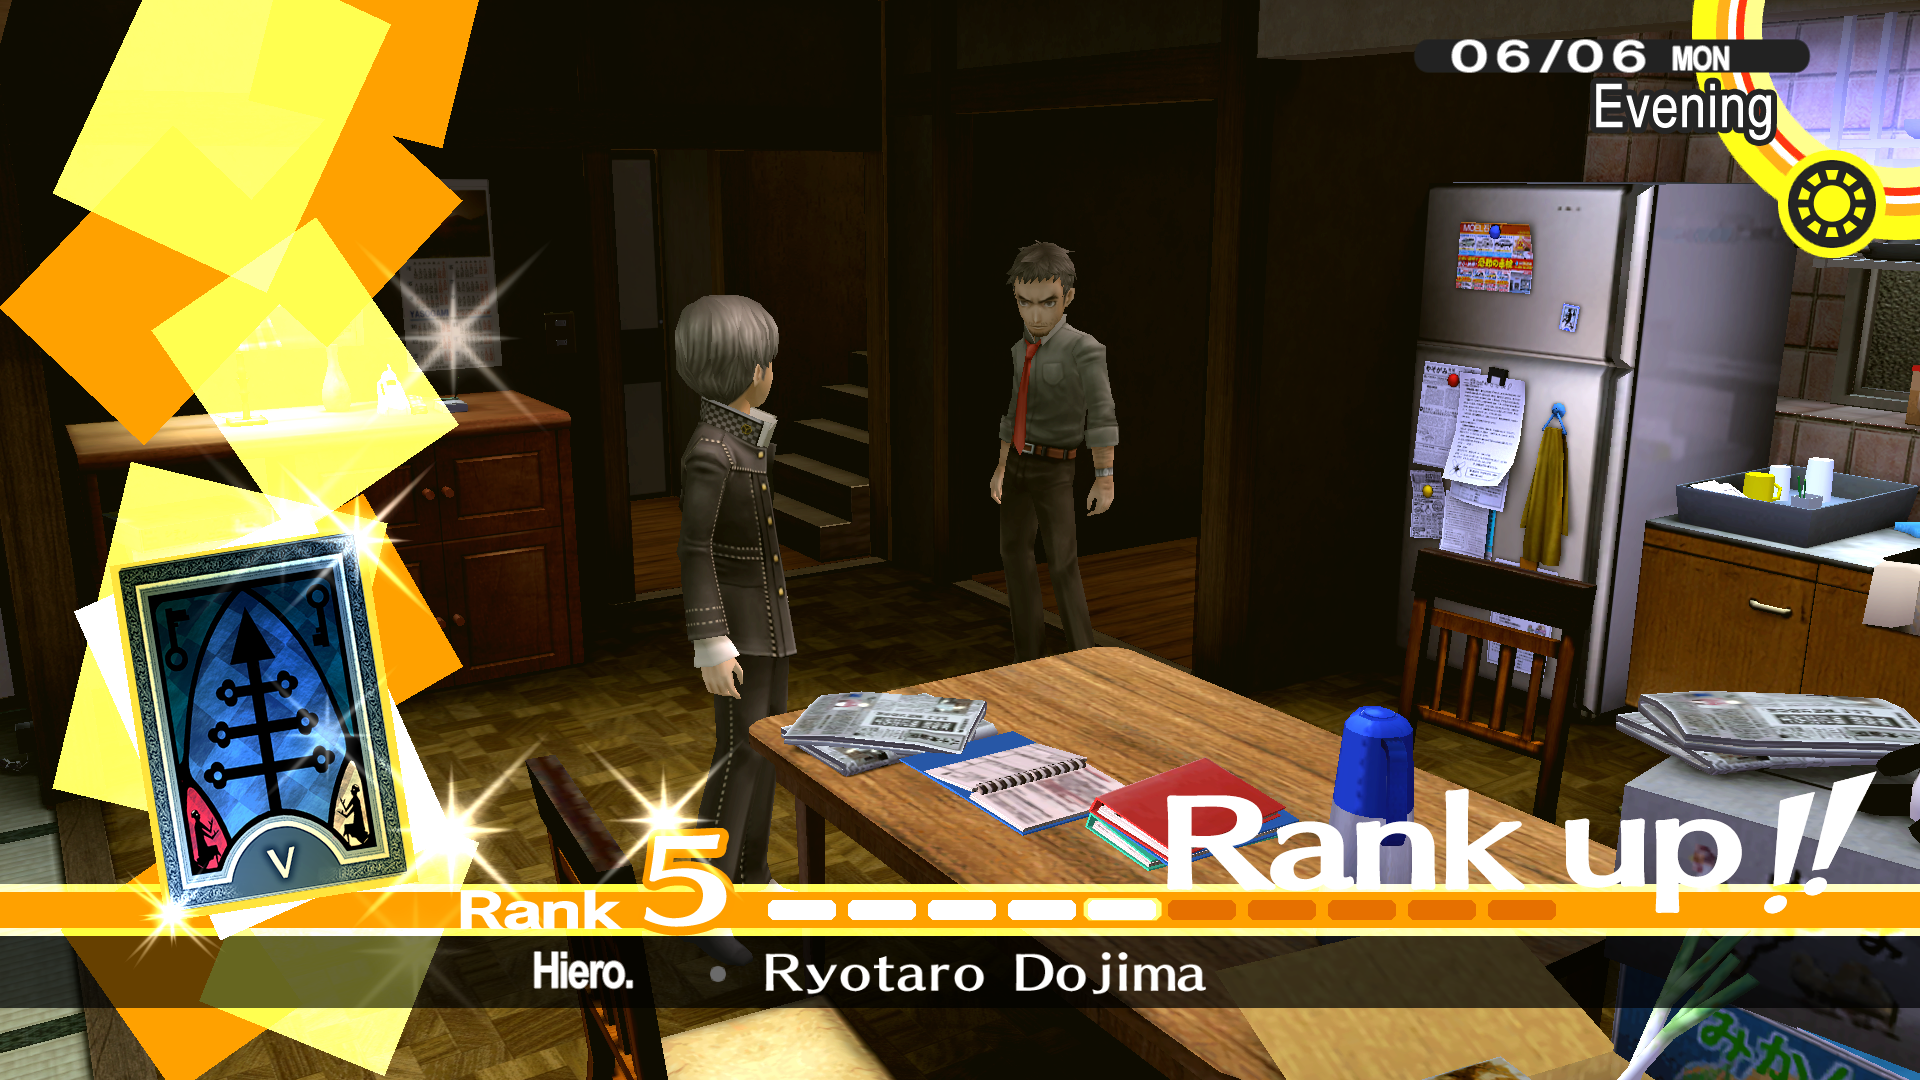
\includegraphics[width=0.8\textwidth]{resources/Dokumentasi/Screenshot (402).png}
              \caption{\label{dojima}Peningkatan Status \textit{Social Link} dengan Ryotaro Dojima}
          \end{figure}
    \item \textit{Social link} setiap karakter dapat ditingkatkan pada hari, waktu, dan lokasi yang berbeda.
    \item Beberapa aksi sepanjang permainan dapat meningkatkan poin \textit{social link} atau \textit{social qualities} yang akan dijelaskan pada \autoref{socialqualities}, seperti menjawab pertanyaan sekolah dan menjawab ujian dengan benar.
    \item Memasak makanan untuk dimakan saat istirahat sekolah dapat meningkatkan poin \textit{social link} dengan karakter lain (lihat \autoref{bentosched}).
    \item Menjawab percakapan karakter lain dengan tepat akan mendapatkan poin yang dapat mempercepat kenaikan \textit{social link} karakter tersebut.
\end{enumerate}


%ini dimasukin ke bab ini juga

%https://gamefaqs.gamespot.com/vita/641695-persona-4-golden/answers/381622-true-ending-requirements-do-i-really-need-to-max-out-all-24-social-links-to

%https://www.rpgsite.net/feature/9824-persona-4-golden-endings-guide-true-ending-requirements-how-to-get-the-canon-end

%Ceritain dari 23 social link ini, yang difokusin di TA ini ada 19 social link karena itu yang ngefek dari 2 alokasi waktunya (done)
Selain faktor-faktor diatas, terdapat cara lain untuk mendapatkan poin tambahan yang dapat mempercepat kenaikan \textit{social link}, yaitu \textit{bonus arcana} dan \textit{bonus} kotak makan siang.

%About Arcana
%https://megamitensei.fandom.com/wiki/Arcana
\textit{Arcana} adalah kelas-kelas yang terdapat pada kartu tarot. Kelas-kelas ini menjadi bagian tematik permainan Persona. Pada pembahasan ini, salah satu asumsi penting yang digunakan ketika meningkatkan \textit{social link} adalah karakter utama memiliki Persona dengan \textit{arcana} yang sama dengan \textit{arcana social link} karakter yang ingin ditingkatkan.

%Makan siang
%https://www.rpgsite.net/feature/9852-persona-4-golden-boxed-lunches-how-to-make-every-perfect-lunch-for-the-cooking-with-gas-achievement --> nanti masukin tutorial nya di lampiran
\textit{Bonus} kotak makan siang adalah \textit{bonus} yang didapatkan dengan membuat bekal pada malam hari untuk dimakan bersama karakter lain pada jam istirahat sekolah keesokan harinya. Jam istirahat sekolah tidak dihitung sebagai aktivitas bebas. Jadi dapat dikatakan bahwa poin \textit{social link} dengan karakter lain dapat bertambah tanpa harus meluangkan waktu beraktivitas bebas (siang dan malam). Namun waktu pembuatan bekal pada malam hari dihitung sebagai satu alokasi waktu bebas karakter utama, sehingga kegiatan pembuatan bekal makan siang sebaiknya dilakukan ketika tidak ada aktivitas yang lebih bermanfaat untuk dilakukan pada hari tersebut.

Jadwal hari yang dapat digunakan untuk membuat bekal pada malam hari dapat dilihat pada \autoref{bentosched}.
\begin{table}[htb]
    \caption{\label{bentosched}Jadwal Pembuatan Bekal}
    \begin{center}
        \begin{tabular}{ | c | c | c | c | c | c |}
            \hline
            \textbf{April} & \textbf{Mei} & \textbf{September} & \textbf{Oktober} & \textbf{November} & \textbf{Januari} \\
            \hline
            25             & 12, 31       & 4, 11, 21, 26, 29  & 25               & 1                 & 11               \\
            \hline
        \end{tabular}
    \end{center}
    %intinya tim investigasi + Marie
\end{table}

%\subsection{\textit{Bonus Arcana}}
%makan siang


\section{Waktu dan Cuaca}
%https://megamitensei.fandom.com/wiki/Weather_Forecast
Dalam permainan P4G, karakter utama memiliki dua alokasi waktu untuk beraktivitas secara bebas, yaitu siang hari dan malam hari. Aktivitas yang dapat dilakukan dan \textit{social link} yang dapat ditingkatkan pada siang dan malam juga berbeda.
Namun, tidak semua hari di Inaba dapat digunakan untuk beraktivitas bebas, karena terdapat hari yang telah dijadwalkan oleh permainan untuk beraktivitas secara otomatis.
Beberapa contoh aktivitas otomatis yang mengakibatkan karakter tidak dapat melakukan aktivitas apapun, yaitu: ujian sekolah, acara sekolah, dan pencarian petunjuk kasus.

%Tambahan (14/07/2023) - Line 80
Waktu bermain Persona 4 Golden adalah selama satu tahun (April 2011 - Maret 2012). Namun, waktu efektif bermain adalah sebanyak 256 hari (April 2011 - Desember 2011) karena setelah bulan Desember 2011 waktu akan berjalan menuju bulan Februari 2012 apabila berhasil memaksimalkan \textit{social link} Marie atau menuju bulan Maret 2012 bagaimanapun kondisi \textit{social link} antara karakter utama dengan seluruh karakter lainnya. Sehingga, dibutuhkan manajemen waktu yang ketat untuk meningkatkan \textit{social link} antara karakter utama dengan 19 karakter lainnya.

Cuaca sangat memengaruhi aktivitas karakter utama selama tinggal di Inaba, karena pada hari dimana karakter tersebut dapat beraktivitas bebas, terdapat batasan aktivitas yang dapat dilakukan pada cuaca tertentu. Jenis-jenis cuaca pada permainan P4G adalah cuaca cerah, cuaca berawan, cuaca hujan, cuaca badai, cuaca berkabut, dan cuaca bersalju. Cuaca dapat dilihat setiap harinya ketika karakter utama memulai aktivitas, televisi di rumah, atau \textit{non player character} (NPC) yang berada di atap sekolah. Kondisi cuaca dalam permainan Persona 4 Golden dapat dilihat pada \autoref{cuaca}.

\begin{figure}[htbp]
    \centering
    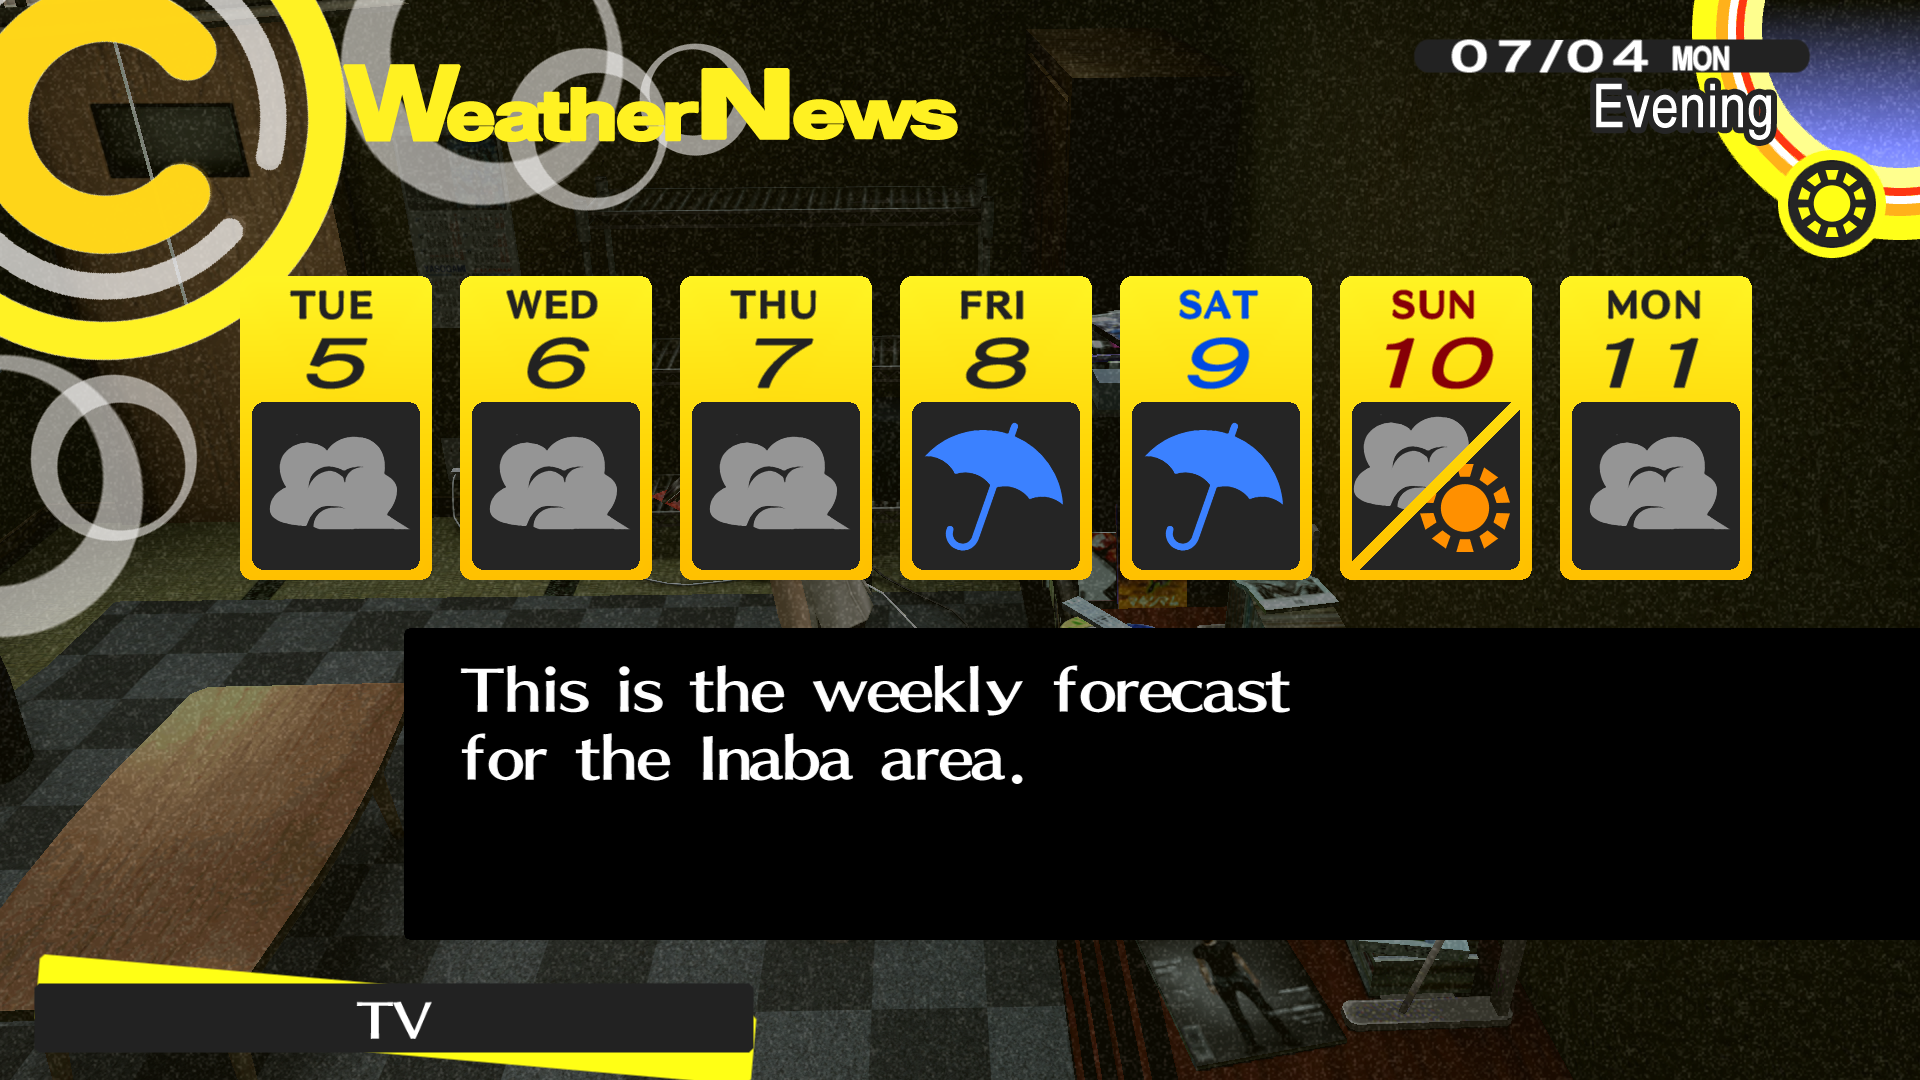
\includegraphics[width=0.8\textwidth]{resources/Dokumentasi/Screenshot (461).png}
    \caption{\label{cuaca}Cuaca di Permainan Persona 4 Golden}
\end{figure}

\subsection{Cuaca Cerah dan Berawan}
Pada cuaca cerah atau berawan, hampir seluruh aktivitas dapat dilakukan. Artinya, pada hari yang sesuai, apabila cuaca cerah atau berawan, karakter utama dapat meningkatkan \textit{social link} dengan karakter. Pada cuaca ini, karakter utama juga dapat bekerja sebagai pengasuh anak untuk mendapatkan gaji serta meningkatkan \textit{social link} dengan Eri Minami.

\subsection{Cuaca Hujan dan Badai}
%https://megamitensei.fandom.com/wiki/Weather_Forecast
Pada cuaca hujan atau badai, hampir seluruh \textit{social link} tidak dapat ditingkatkan. Akan tetapi, terdapat aktivitas-aktivitas yang mendapatkan \textit{bonus} atau hanya dapat dilakukan ketika dilakukan pada cuaca ini, seperti:
\begin{enumerate}
    \item Belajar, \textit{social qualities "Knowledge"} akan meningkat dua kali lipat.
    \item Makan \textit{Mega Beef Bowl} seharga 3.000 yen di \textit{The Chinese Diner Aiya} akan meningkatkan \textit{Social qualities "Understanding", "Knowledge", "Diligence"} dan \textit{"Courage"}.
    \item Belanja di \textit{Shiroku Store} akan mendapatkan diskon 50\%.
    \item \textit{Shiroku Store Capsule Machine} dapat digunakan.
    \item \textit{Deidara Metalworks} akan tetap buka dan menawarkan diskon pada malam hujan.
    \item \textit{Super croquettes} dapat dibeli maksimal sebanyak lima di \textit{Souzai Daigaku}.
    \item Ikan yang lebih menantang lebih sering muncul di \textit{Samegawa Flood Plain} dan \textit{Shichiri Beach}.
    \item Kegiatan menangkap serangga di \textit{Tatsuhime Shrine} tidak dapat dilakukan.
    \item Beberapa \textit{shadows} di \textit{Midnight Channel} hanya muncul pada cuaca hujan.
    \item Peluang \textit{shadows} menghasilkan benda langka lebih besar.
    \item \textit{Skill rainy death} mengalami peningkatan \textit{critical rate} pada cuaca hujan.
    \item Hampir seluruh \textit{social link} tidak dapat ditingkatkan, kecuali Ayane Matsunaga/Yumi Ozawa, Fox, Nanako Dojima, Ryotaro Dojima, Sayoko Uehara, dan Shu Nakajima.
    \item Hampir seluruh misi \textit{outdoor} NPC tidak ada.
    \item Membaca buku di rumah karakter utama pada cuaca hujan dapat meningkatkan lebih banyak \textit{social qualities}.
\end{enumerate}

\subsection{Cuaca Berkabut}
Cuaca berkabut menggambarkan batas waktu menyelesaikan \textit{dungeon}. Ketika karakter utama memiliki misi menyelamatkan karakter lain dalam \textit{dungeon}, misi tersebut harus diselesaikan sebelum cuaca hujan tiga hari berturut-turut. Apabila \textit{dungeon} tidak berhasil diselesaikan sebelum cuaca berkabut, artinya permainan gagal diselesaikan.

\subsection{Cuaca Bersalju}
%https://megamitensei.fandom.com/wiki/Weather_Forecast
Cuaca bersalju hampir sama seperti cuaca cerah atau berawan. Namun, aktivitas seperti berkebun dan menangkap serangga tidak dapat dilakukan. Sebagai tambahan, karakter utama dapat mencari serangga dengan menggali salju di kebun rumah Dojima. Perlu diperhatikan bahwa aktivitas-aktivitas diatas tidak akan meningkatkan \textit{social qualities} atau \textit{social link}, hanya akan menambah benda yang dimiliki karakter utama.


\section{\label{socialqualities}\textit{Social Qualities}}
%https://www.rpgsite.net/feature/9822-persona-4-golden-part-time-jobs-every-job-requirements-rewards
%https://www.rpgsite.net/feature/9823-persona-4-golden-social-stats-raising-knowledge-courage-expression-diligence-understanding
\textit{Social qualities} adalah status yang menggambarkan keadaan karakter utama. Berdasarkan jenisnya, \textit{social qualities} dibagi menjadi lima, yaitu: \textit{Knowledge}, \textit{Courage}, \textit{Expression}, \textit{Diligence}, dan \textit{Understanding}.
%\textit{Social qualities} dapat dilihat pada \autoref{socialstats}.


\begin{figure}[htbp]
    \centering
    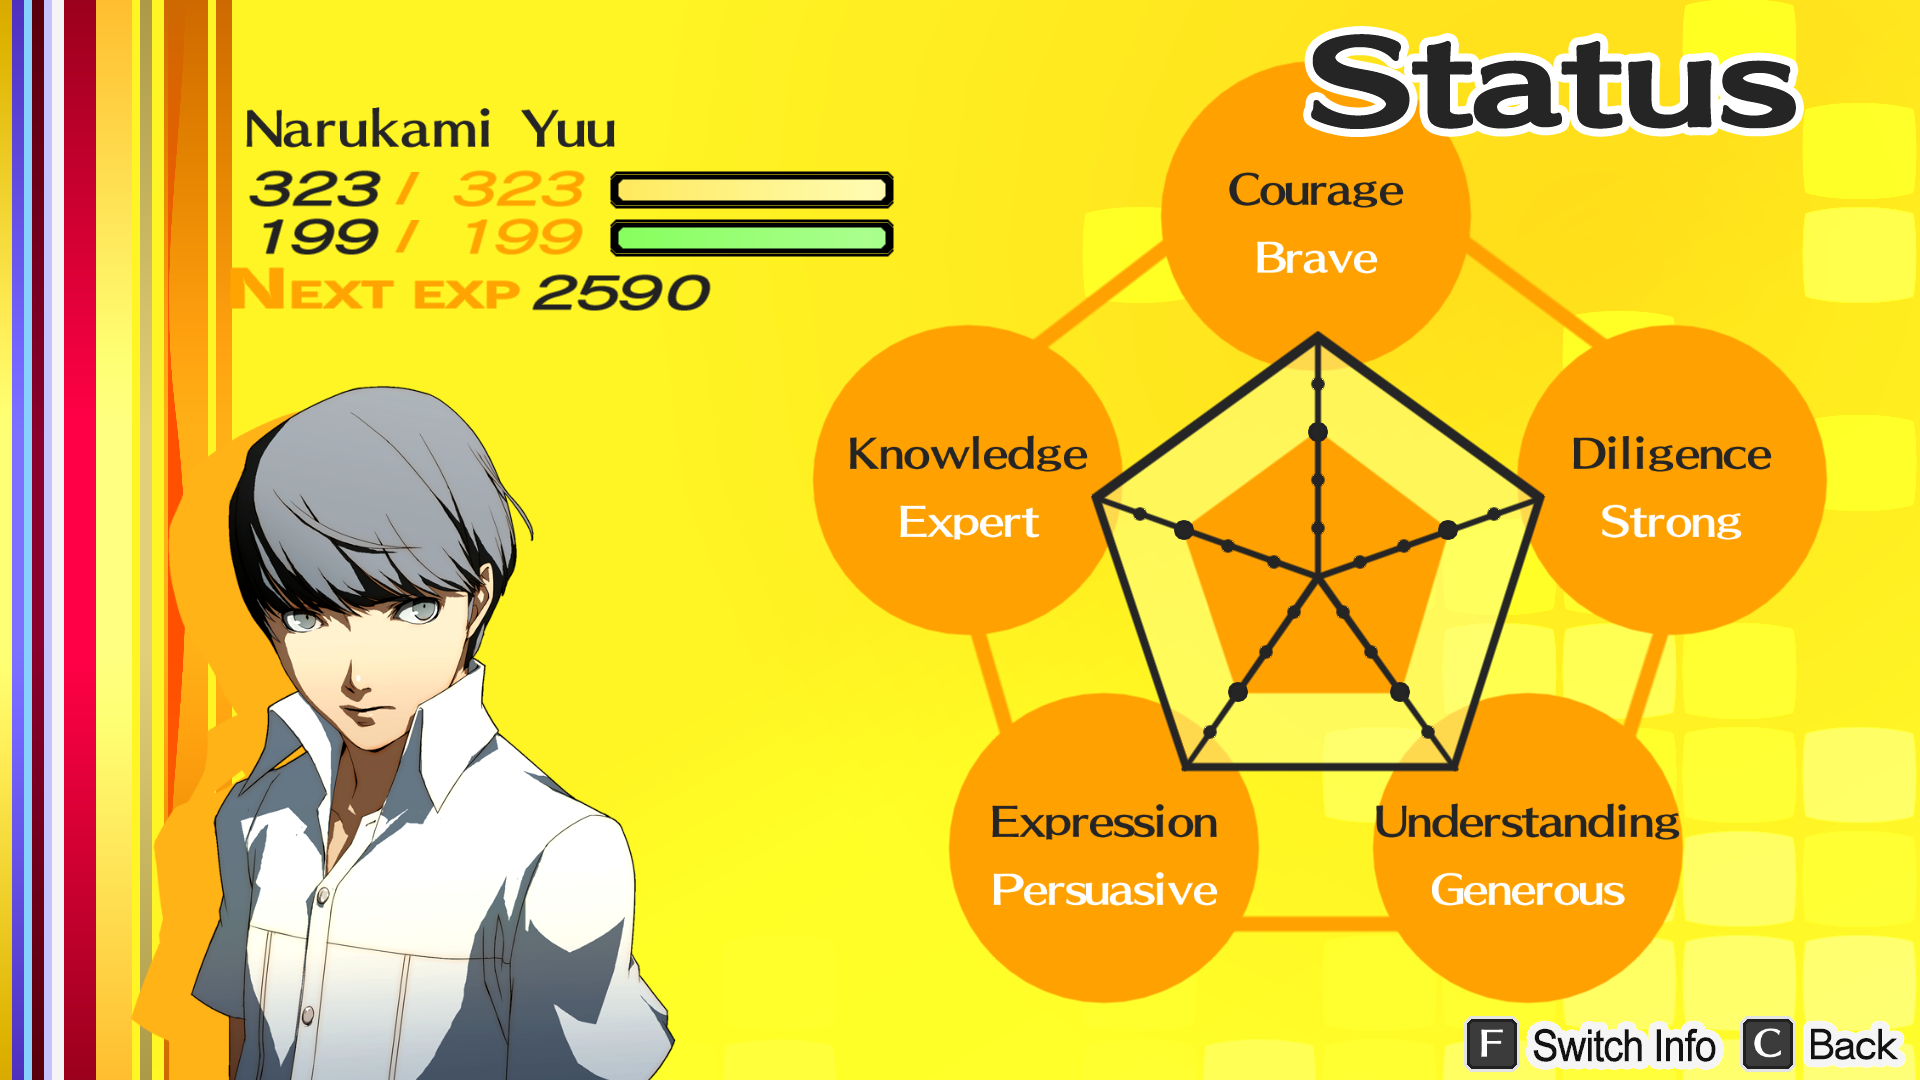
\includegraphics[width=0.8\textwidth]{resources/Dokumentasi/Screenshot (460).png}
    \caption{\label{socialstats}Status \textit{Social Qualities}}
\end{figure}

Status \textit{social qualities} dapat dilihat pada \autoref{socialstats}. Perlu diperhatikan bahwa jumlah poin yang harus didapatkan untuk meningkatkan setiap jenis \textit{social qualities} berbeda-beda. \textit{Social qualities} perlu ditingkatkan karena untuk meningkatkan \textit{social link} beberapa karakter, dibutuhkan persyaratan \textit{social qualities}.

%Knowledge
\subsection{\textit{Knowledge}}
Status \textit{Knowledge} merepresentasikan level pengetahuan karakter utama. Ketika karakter utama mendapatkan hasil yang sangat baik dalam ujian, karakter utama mendapatkan hadiah tambahan.

Level \textit{Knowledge} tertentu dibutuhkan untuk memulai \textit{social link} dengan karakter-karakter berikut:
\begin{itemize}
    \item Margaret (\textit{Empress}). Level \textit{Knowledge}: \textit{Expert}.
    \item Naoto Shirogane (\textit{Fortune}). Level \textit{Knowledge}: \textit{Sage}.
\end{itemize}

Jumlah poin yang dibutuhkan untuk meningkatkan \textit{Knowledge} karakter utama dapat dilihat pada \autoref{knowlevel}.
\begin{table}[H]
    \caption{\label{knowlevel}Sistem Poin Status \textit{Knowledge}}
    \begin{center}
        \begin{tabular}{ | c | c | c | c | c | }
            \hline
            \textbf{Level 1} & \textbf{Level 2}  & \textbf{Level 3} & \textbf{Level 4}   & \textbf{Level 5} \\
            \hline
            \textit{Aware}   & \textit{Informed} & \textit{Expert}  & \textit{Professor} & \textit{Sage}    \\
            \hline
            $\le$ 29 poin    & 30-79 poin        & 80-149 poin      & 150-239 poin       & $\ge$ 240 poin   \\
            \hline
        \end{tabular}
    \end{center}
\end{table}

Terdapat beberapa cara yang dapat dilakukan untuk meningkatkan status \textit{Knowledge}, seperti:
\begin{enumerate}
    \item Menjawab pertanyaan di kelas secara benar. %+3 poin
    \item Membaca buku: \textit{The Gentle Way, The Punk’s Way, Guide to Pests, Poly-land, The O-Cha Way, The Divine Way, Who Am I} dan \textit{The Ramen Way}. %https://www.ign.com/wikis/shin-megami-tensei-persona-4-golden/Books
    \item Membaca buku \textit{Expert Study Methods} dapat meningkatkan jumlah poin \textit{Knowledge} yang didapat saat belajar.
    \item Belajar di rumah pada malam hari. %+3 poin
    \item Belajar di perpustakaan sekolah pada siang hari.  %+3 poin kl sendiri, kalo bareng gatau
    \item Makan siang di \textit{The Chinese Diner Aiya} pada cuaca hujan.
\end{enumerate}

%Courage
\subsection{\textit{Courage}}
Status \textit{Courage} merepresentasikan level keberanian karakter utama. Dalam beberapa percakapan dengan karakter lain, dibutuhkan level keberanian yang lebih tinggi.

Level \textit{Courage} tertentu dibutuhkan untuk memulai \textit{social link} dengan karakter-karakter berikut:
\begin{itemize}
    \item Ai Ebihara (\textit{Moon}). Level \textit{Courage}: \textit{Brave}.
    \item Naoto Shirogane (\textit{Fortune}). Level \textit{Courage}: \textit{Heroic}.
\end{itemize}

Jumlah poin yang dibutuhkan untuk meningkatkan \textit{Courage} karakter utama dapat dilihat pada \autoref{coulevel}.
\begin{table}[H]
    \caption{\label{coulevel}Sistem Poin Status \textit{Courage}}
    \begin{center}
        \begin{tabular}{ | c | c | c | c | c | }
            \hline
            \textbf{Level 1} & \textbf{Level 2}  & \textbf{Level 3} & \textbf{Level 4} & \textbf{Level 5} \\
            \hline
            \textit{Average} & \textit{Reliable} & \textit{Brave}   & \textit{Daring}  & \textit{Heroic}  \\
            \hline
            $\le$ 15 poin    & 16-39 poin        & 40-79 poin       & 80-139 poin      & $\ge$ 140 poin   \\
            \hline
        \end{tabular}
    \end{center}
\end{table}

\begin{figure}[htbp]
    \centering
    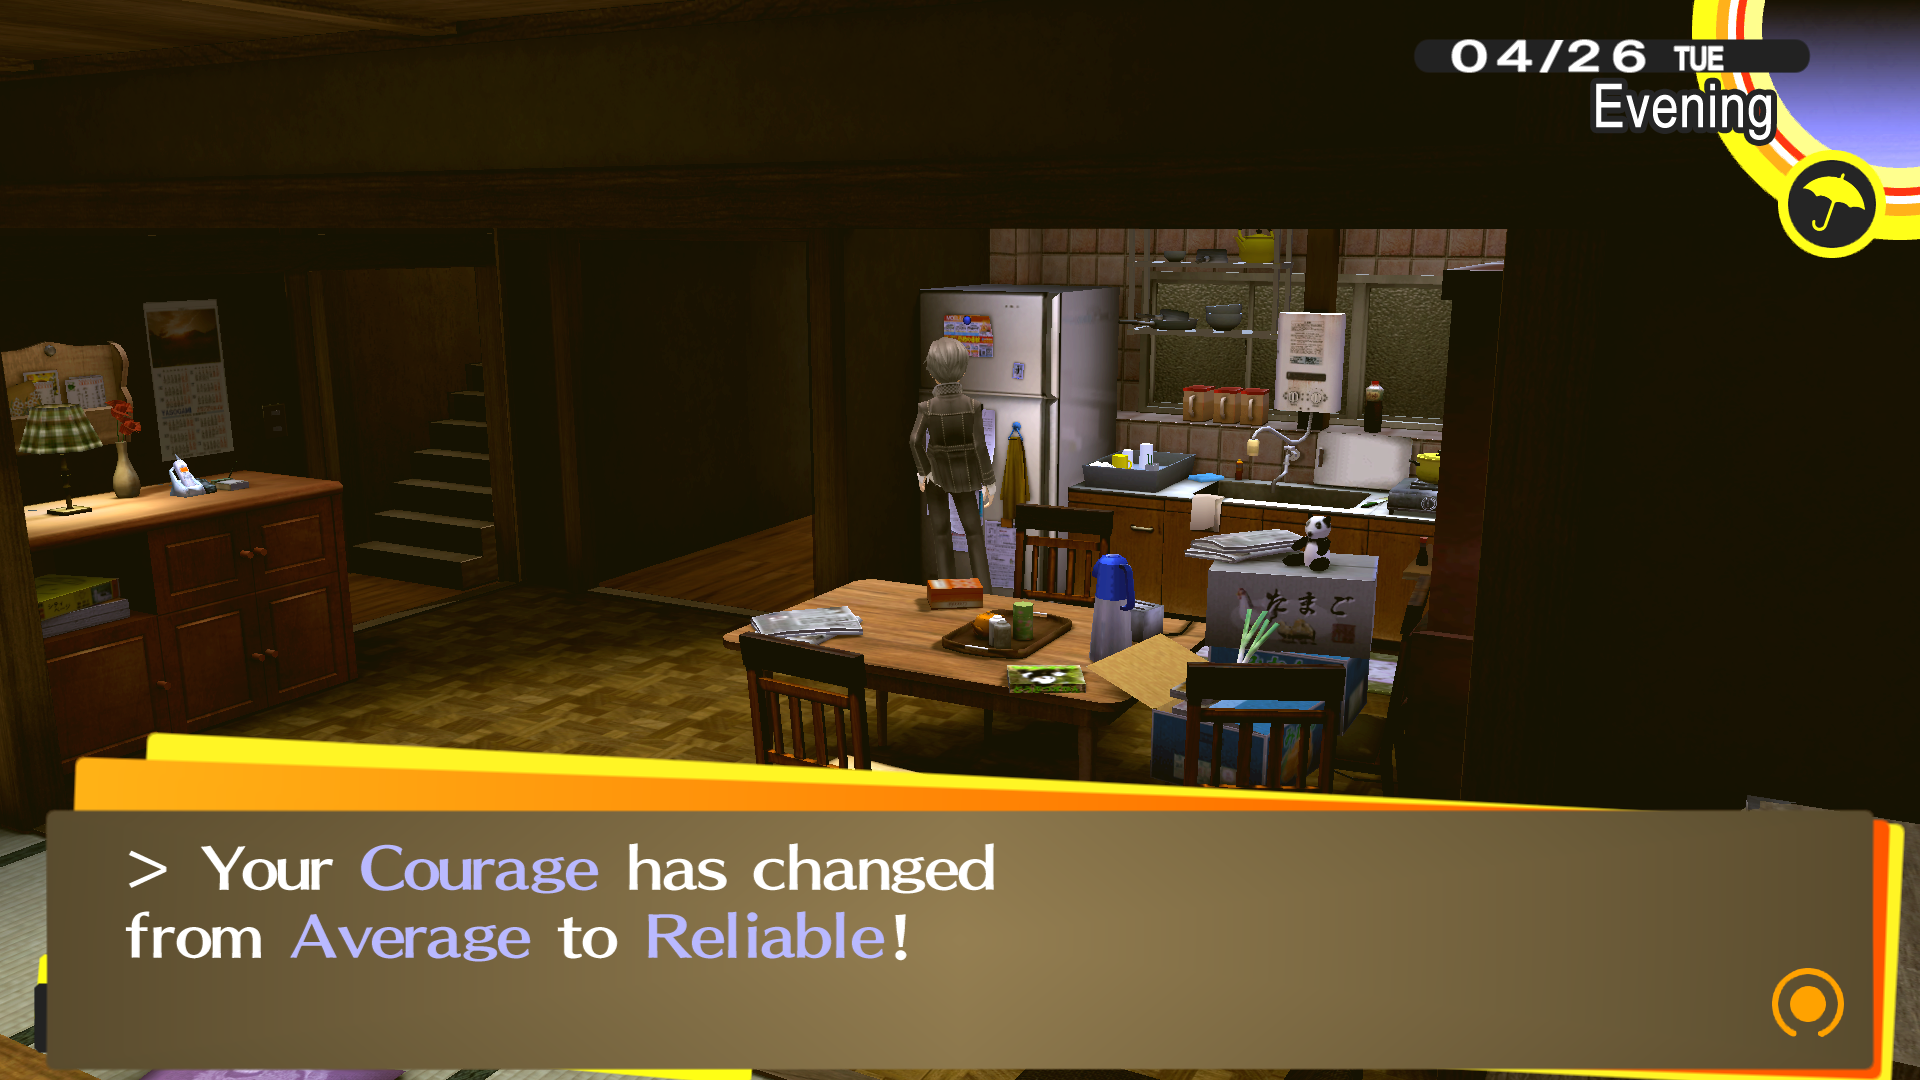
\includegraphics[width=0.8\textwidth]{resources/Dokumentasi/Screenshot (381).png}
    \caption{\label{courage}Peningkatan Level Status \textit{Social Qualities Courage}}
\end{figure}

Terdapat beberapa cara yang dapat dilakukan untuk meningkatkan status \textit{Courage}, seperti:
\begin{enumerate}
    \item Makan siang di \textit{The Chinese Diner Aiya} pada 19 April 2011 dan pada cuaca hujan.
    \item Makan malam di kulkas rumah pada hari-hari tertentu. Jadwal tersebut dapat dilihat pada \autoref{kulkas}. Gambar peningkatan status \textit{courage} dapat dilihat pada \autoref{courage}.
    \item Bekerja paruh waktu di rumah sakit pada malam hari.
    \item Membaca buku: \textit{The Lovely Man, Forever Macho, Guide to Pests, Man of History, Man-God}, dan \textit{Farewell to Man.}
    \item Mengendarai motor.
    \item Mengalahkan \textit{boss dungeon} opsional.
\end{enumerate}

Pada hari-hari tertentu, karakter utama dapat makan makanan kulkas di rumah Dojima dan meningkatkan status \textit{Courage}. Jadwal tersebut dapat dilihat pada \autoref{kulkas}
\begin{table}[htb]
    \caption{\label{kulkas}Jadwal Meningkatkan Status \textit{Courage} Melalui Kulkas Dojima}
    \begin{center}
        \begin{tabular}{ | c | c | c | c | c | c | c | }
            \hline
            \textbf{April} & \textbf{Mei} & \textbf{Juni} & \textbf{Juli} & \textbf{Agustus} & \textbf{September} & \textbf{Oktober} \\
            \hline
            25             & 2, 14, 30    & 20            & 4, 18         & 29               & 13                 & 24               \\
            \hline
        \end{tabular}
    \end{center}
\end{table}

%Expression
\subsection{\textit{Expression}}
Status \textit{Expression} merepresentasikan level ekspresi karakter utama. Semakin tinggi level ekspresi karakter utama, semakin banyak opsi percakapan yang dimiliki karakter utama.

Level \textit{Expression} tertentu dibutuhkan untuk memulai \textit{social link} dengan karakter-karakter berikut:
\begin{itemize}
    \item{Ryotaro Dojima (\textit{Hierophant}). Level \textit{Expression}:
                \begin{enumerate}
                    \item \textit{Eloquent}, untuk meningkatkan \textit{social link} level 1 ke level 2.
                    \item \textit{Persuasive}, untuk meningkatkan \textit{social link} level 3 ke level 4.
                    \item \textit{Touching}, untuk meningkatkan \textit{social link} level 4 ke level 5.
                \end{enumerate}
          }
    \item{Nanako Dojima (\textit{Justice}).
                Level \textit{Expression}:
                \begin{enumerate}
                    \item \textit{Persuasive}, untuk meningkatkan \textit{social link} level 3 ke level 4.
                    \item \textit{Enthrailling}, untuk meningkatkan \textit{social link} level 5 ke level 6.
                \end{enumerate}
          }
\end{itemize}

Jumlah poin yang dibutuhkan untuk meningkatkan \textit{Expression} karakter utama dapat dilihat pada \autoref{exlevel}.
\begin{table}[H]
    \caption{\label{exlevel}Sistem Poin Status \textit{Expression}}
    \begin{center}
        \begin{tabular}{ | c | c | c | c | c | }
            \hline
            \textbf{Level 1} & \textbf{Level 2}  & \textbf{Level 3}    & \textbf{Level 4}  & \textbf{Level 5}      \\
            \hline
            \textit{Rough}   & \textit{Eloquent} & \textit{Persuasive} & \textit{Touching} & \textit{Enthrailling} \\
            \hline
            $\le$ 12 poin    & 13-32 poin        & 33-52 poin          & 53-84 poin        & $\ge$ 85 poin         \\
            \hline
        \end{tabular}
    \end{center}
\end{table}

Terdapat beberapa cara yang dapat dilakukan untuk meningkatkan status \textit{Expression}, seperti:
\begin{enumerate}
    \item Bekerja paruh waktu sebagai guru les pada malam hari.
    \item Bekerja paruh waktu sebagai penerjemah pada malam hari.
    \item Menjawab pertanyaan tertentu dari guru sekolah.
    \item Membaca buku: \textit{The Gentle Way, English Made Easy, The Punk’s Way, The O-Cha Way}, dan \textit{The Divine Way}.
    \item Mengikuti klub drama.
          %https://www.rpgsite.net/feature/9883-persona-4-basketball-vs-soccer-music-vs-drama-which-school-clubs-to-choose
\end{enumerate}

%Diligence
\subsection{\textit{Diligence}}
Status \textit{Diligence} merepresentasikan level kerajinan karakter utama. Karakter utama memiliki opsi aktivitas baru ketika level kerajinannya semakin tinggi.

Level \textit{Diligence} tertentu dibutuhkan untuk memulai \textit{social link} dengan karakter berikut:
\begin{itemize}
    \item Sayoko Uehara (\textit{Devil}). Level \textit{Diligence}: \textit{Strong}.
\end{itemize}

Jumlah poin yang dibutuhkan untuk meningkatkan \textit{Diligence} karakter utama dapat dilihat pada \autoref{dililevel}.
\begin{table}[H]
    \caption{\label{dililevel}Sistem Poin Status \textit{Diligence}}
    \begin{center}
        \begin{tabular}{ | c | c | c | c | c | }
            \hline
            \textbf{Level 1} & \textbf{Level 2}    & \textbf{Level 3} & \textbf{Level 4}    & \textbf{Level 5}    \\
            \hline
            \textit{Callow}  & \textit{Persistent} & \textit{Strong}  & \textit{Persuasive} & \textit{Rock Solid} \\
            \hline
            $\le$ 15 poin    & 16-39 poin          & 40-79 poin       & 80-139 poin         & $\ge$ 140 poin      \\
            \hline
        \end{tabular}
    \end{center}
\end{table}

Terdapat beberapa cara yang dapat dilakukan untuk meningkatkan status \textit{Diligence}, seperti:
\begin{enumerate}
    %https://www.rpgsite.net/feature/9823-persona-4-golden-social-stats-raising-knowledge-courage-expression-diligence-understanding
    \item Membaca buku: \textit{ Witch Detective, Poly-land, Picross Rules!}, dan \textit{Who am I?}
    \item Membaca buku \textit{Office Work Manual} dapat meningkatkan jumlah poin \textit{Diligence} yang didapat saat bekerja sebagai pembuat kertas surat.
    \item Bekerja paruh waktu sebagai pembuat kertas surat pada malam hari.
    \item Bekerja paruh waktu di bar pada malam hari.
    \item Mengikuti klub olahraga.
    \item Mengerjakan \textit{unfinished models} 1 dan 2.
    \item Berkebun di kebun rumah Dojima.
    \item Makan siang di \textit{The Chinese Diner Aiya} pada cuaca hujan.
\end{enumerate}

%Understanding
\subsection{\textit{Understanding}}
Status \textit{Understanding} merepresentasikan level penalaran karakter utama. Karakter utama memiliki opsi aktivitas baru ketika level penalarannya semakin tinggi.

Level \textit{Understanding} tertentu dibutuhkan untuk memulai \textit{social link} dengan karakter berikut:
\begin{itemize}
    \item Naoki Konishi (\textit{Hanged Man}). Level \textit{Understanding}: \textit{Generous}.
    \item Shu Nakajima (\textit{Tower}). Level \textit{Understanding}: \textit{Saintly}.
\end{itemize}

Jumlah poin yang dibutuhkan untuk meningkatkan \textit{Understanding} karakter utama dapat dilihat pada \autoref{underlevel}.
\begin{table}[H]
    \caption{\label{underlevel}Sistem Poin Status \textit{Understanding}}
    \begin{center}
        \begin{tabular}{ | c | c | c | c | c | }
            \hline
            \textbf{Level 1} & \textbf{Level 2} & \textbf{Level 3}  & \textbf{Level 4}  & \textbf{Level 5} \\
            \hline
            \textit{Basic}   & \textit{Kindly}  & \textit{Generous} & \textit{Motherly} & \textit{Saintly} \\
            \hline
            $\le$ 15 poin    & 16-39 poin       & 40-79 poin        & 80-139 poin       & $\ge$ 140 poin   \\
            \hline
        \end{tabular}
    \end{center}
\end{table}
%naikin eri minami bisa dapat understanding

Terdapat beberapa cara yang dapat dilakukan untuk meningkatkan status \textit{Understanding}, seperti:
\begin{enumerate}
    %https://www.rpgsite.net/feature/9823-persona-4-golden-social-stats-raising-knowledge-courage-expression-diligence-understanding
    %https://www.ign.com/wikis/shin-megami-tensei-persona-4-golden/Social_Qualities
    \item Membaca buku: \textit{Off Today, Witch Detective, Short on Cash, Changing Careers, Picross Rules, Sensei’s Friends, The Final Lesson}, dan \textit{The Ramen Way}.
    \item Membaca buku \textit{Easy Origami Book} dapat meningkatkan jumlah poin \textit{Understanding} yang didapat saat bekerja sebagai pelipat origami.
    \item Bekerja paruh waktu sebagai pelipat origami pada malam hari.
    \item Bekerja paruh waktu sebagai penjaga anak pada siang hari.
    \item Menghabiskan waktu bersama kucing pada malam hari.
    \item Membersihkan ruangan setelah latihan sepak bola (klub olahraga).
    \item Makan siang di \textit{The Chinese Diner Aiya} pada cuaca hujan.
\end{enumerate}

Untuk peningkatan status \textit{social qualities}, akan terlihat tulisan \textit{"Your Understanding has increased} seperti pada \autoref{SL}. Tulisan \textit{understanding} dapat digantikan dengan status \textit{social qualities} lainnya.
\begin{figure}[htbp]
    \centering
    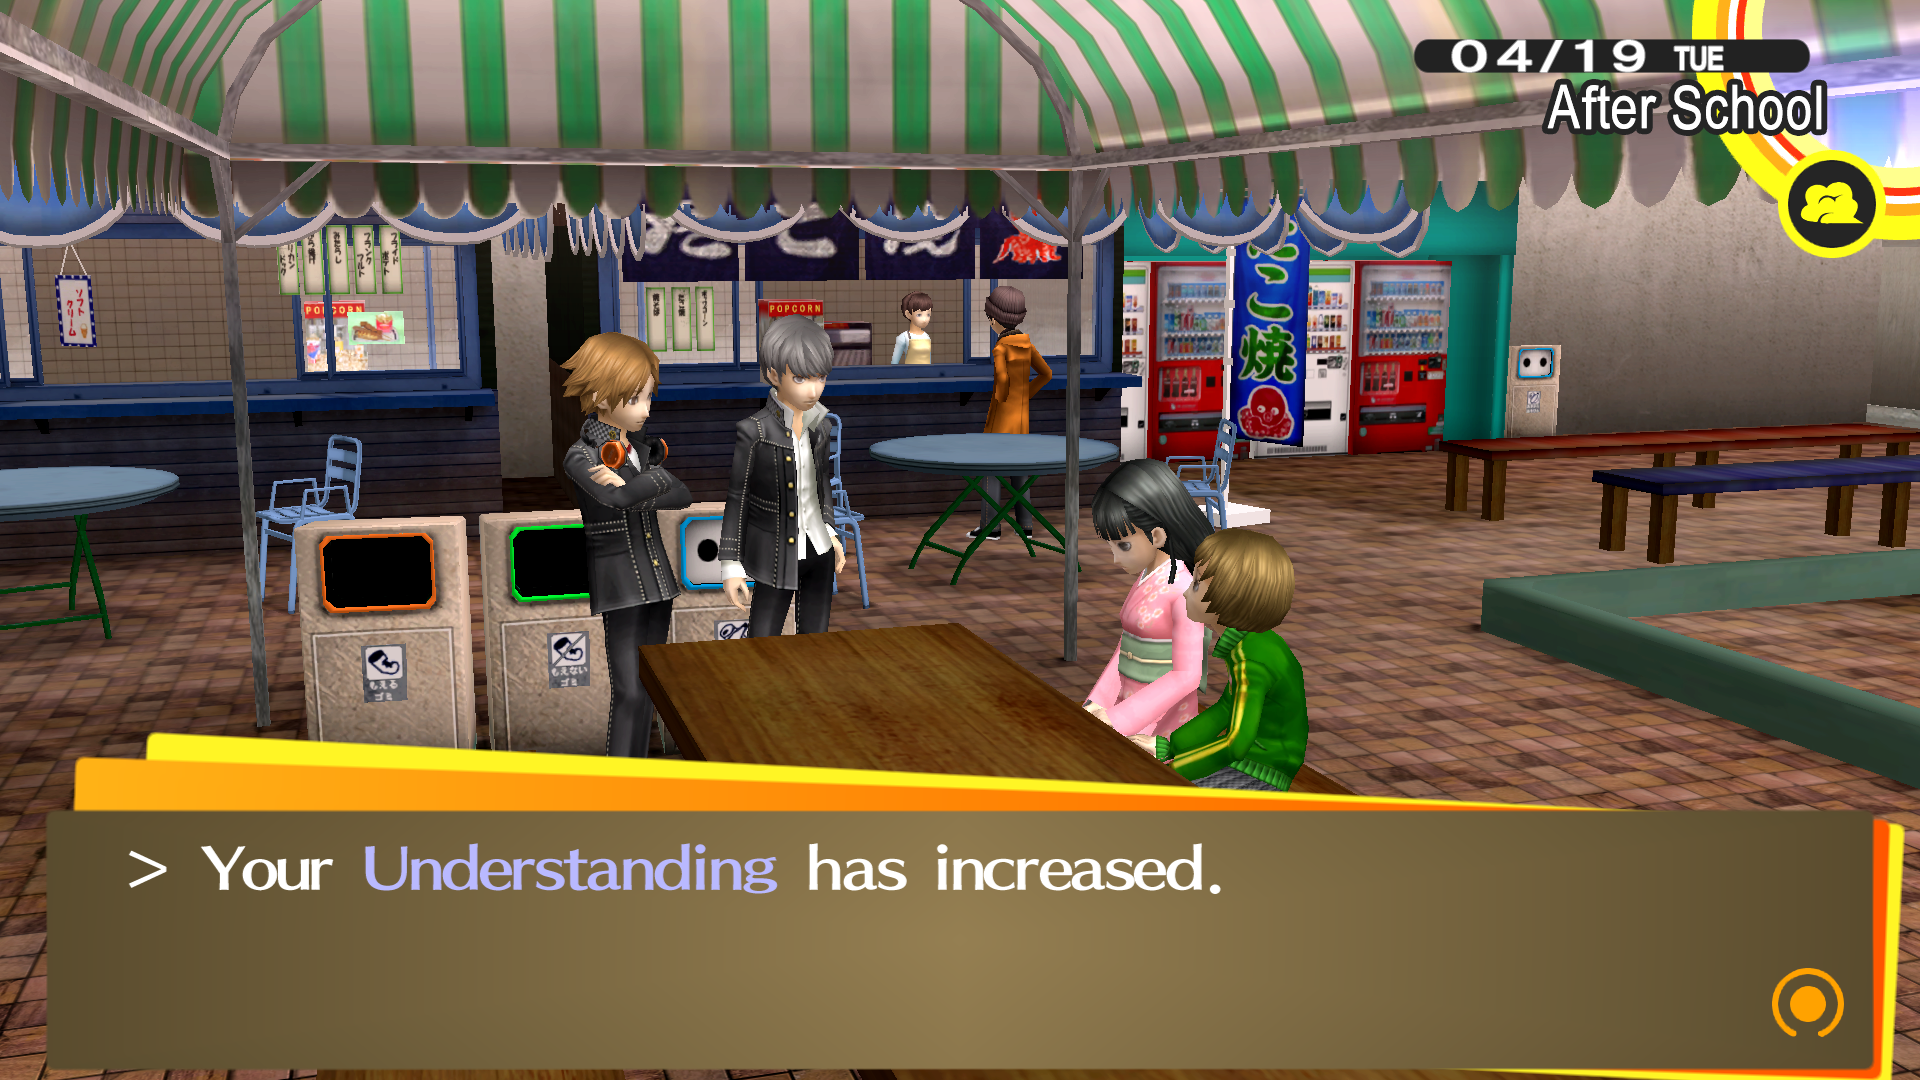
\includegraphics[width=0.8\textwidth]{resources/Dokumentasi/Screenshot (379).png}
    \caption{\label{SL}Peningkatan Status \textit{Social Qualities Understanding}}
\end{figure}

\section{Perkembangan Kasus}
%https://steamcommunity.com/sharedfiles/filedetails/?id=2156615735
Salah satu variabel utama yang memengaruhi jadwal peningkatan \textit{social link} adalah ketika karakter utama sedang menginvestigasi kasus atau menyelesaikan kasus.

\subsection{Mode Investigasi}
Pada mode ini, karakter utama harus mencari petunjuk untuk kasus yang ingin diselesaikan. Apabila karakter utama belum menemukan seluruh petunjuk kasus, \textit{social link} karakter-karakter dibawah ini tidak dapat ditingkatkan.
\begin{table}[htb]
    \caption{\label{investigationmode}\textit{Social Link} yang Tidak Dapat Ditingkatkan pada Mode Investigasi}
    \begin{center}
        \begin{tabular}{ | c | c | c |}
            \hline
            \textbf{No} & \textbf{Nama Karakter} & \textbf{Arcana} \\
            \hline
            1.          & Yosuke Hanamura        & Magician        \\
            \hline
            2.          & Chie Satonaka          & Chariot         \\
            \hline
            3.          & Yukiko Amagi           & Priestess       \\
            \hline
            4.          & Kanji Tatsumi          & Emperor         \\
            \hline
            5.          & Rise Kujikawa          & Lovers          \\
            \hline
            6.          & Naoto Shirogane        & Fortune         \\
            \hline
            7.          & Marie                  & Aeon            \\
            \hline
        \end{tabular}
    \end{center}
    %intinya tim investigasi + Marie
\end{table}


\subsection{Mode Eksplorasi}
Setelah menginvestigasi kasus dan mendapatkan petunjuk, karakter utama harus menyelesaikan kasus dengan mengeksplorasi \textit{dungeon}. Pada waktu ini, \textit{social link} beberapa karakter (anggota tim kasus) tidak dapat ditingkatkan hingga \textit{dungeon} telah selesai dieksplorasi, atau kasus telah diselesaikan.

\begin{figure}[htbp]
    \centering
    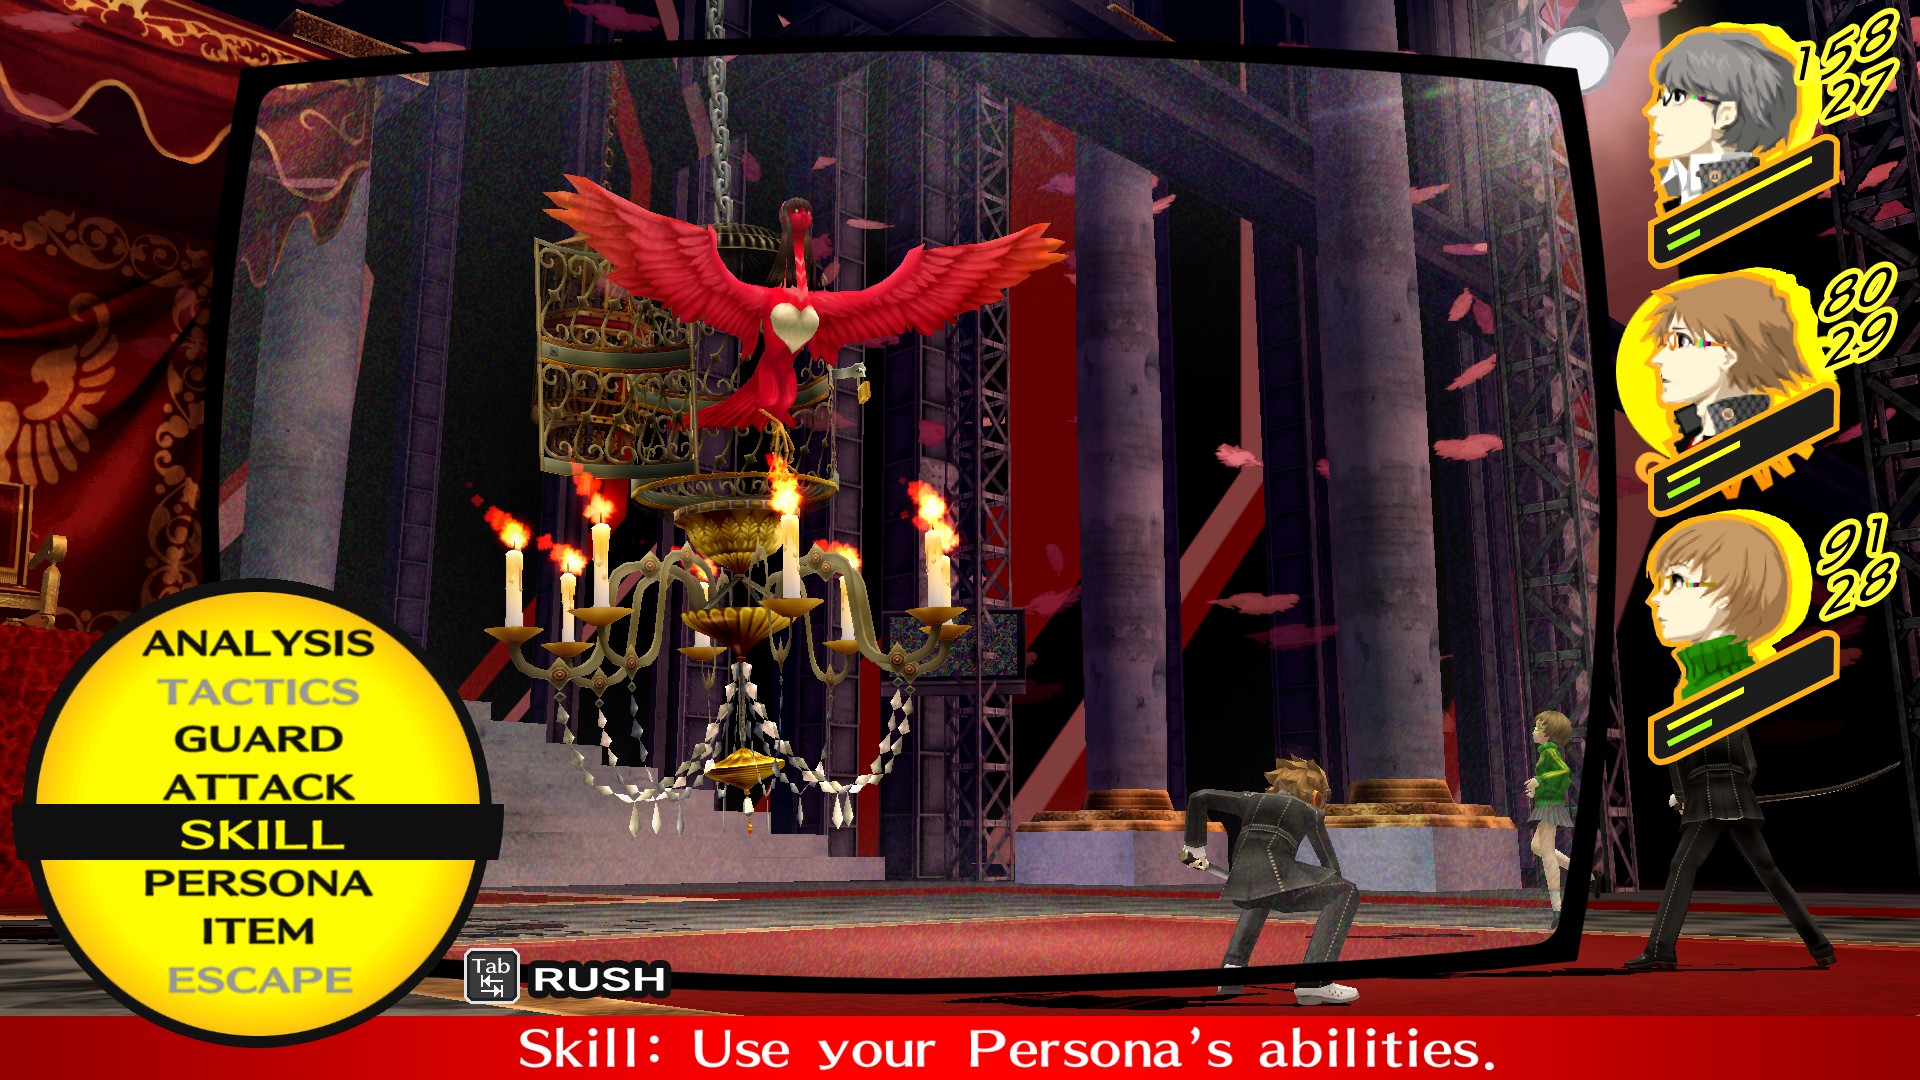
\includegraphics[width=0.8\textwidth]{resources/Dokumentasi/Screenshot (377).png}
    \caption{\label{dungeon}Mode Eksplorasi Permainan Persona 4 Golden}
\end{figure}

Selain itu perhatikan pula untuk karakter Ryotaro Dojima, apabila karakter utama menyelesaikan \textit{dungeon} lebih awal, Ryotaro Dojima akan memiliki waktu luang lebih pada malam hari sehingga karakter utama memiliki lebih banyak waktu untuk meningkatkan level \textit{social link} dengan Ryotaro Dojima. Namun, perlu diperhatikan bahwa ketika Ryotaro Dojima ada di rumah, level \textit{social link} karakter Nanako Dojima tidak dapat ditingkatkan. \textit{Social link} Nanako Dojima hanya dapat ditingkatkan ketika Ryotaro Dojima sedang bertugas atau tidak ada di rumah.


\section{Simulasi Permainan Persona 4 Golden}
Ketika menyimulasikan interaksi sosial yang terjadi dalam permainan Persona 4 Golden, perhatikan bahwa hanya terdapat satu karakter yang dimainkan oleh pemain, yaitu karakter utama. Simulasi yang dilakukan bertujuan untuk mencari jadwal terbaik ketika meningkatkan hubungan sosial antara karakter utama dengan seluruh karakter. Maka, aksi dan keluaran merupakan strategi pemilihan jadwal terbaik untuk meningkatkan \textit{social link} dengan seluruh karakter lain berdasarkan preferensi. Definisikan aksi, \textit{payoff}, dan preferensi pemain dalam simulasi permainan Persona 4 Golden sebagai berikut:

\begin{enumerate}
    \item \textbf{Aksi:} Memilih karakter untuk ditingkatkan \textit{social link}-nya.
    \item \textbf{Preferensi:} Karakter yang ditingkatkan \textit{social link}-nya pada suatu hari merupakan karakter dengan bobot \textit{payoff} terbesar.
    \item \textbf{\textit{Payoff:}} Dijelaskan pada bagian selanjutnya.
\end{enumerate}

Sekarang, akan dibahas lebih lanjut mengenai matriks \textit{payoff}. Matriks \textit{payoff} simulasi yang dilakukan adalah matriks diagonal A berukuran 19 x 19 yang menggambarkan status \textit{social link} awal seluruh karakter dalam permainan Persona 4 Golden dengan $a_{ii}$ merupakan status \textit{social link} suatu karakter, nilai $i = 1,2,...,19, i$ adalah jumlah karakter yang perlu ditingkatkan status \textit{social link}-nya.

\[
    A =
    \begin{bmatrix}
        a_{1,1} & 0       & \cdots & 0         \\
        0       & a_{2,2} & \ddots & \vdots    \\
        \vdots  & \ddots  & \ddots & 0         \\
        0       & \cdots  & 0      & a_{19,19}
    \end{bmatrix}
\]

Perhatikan bahwa \textit{social link} setiap karakter dapat ditingkatkan sebanyak 10 level, sehingga definisikan $a_{ii}= 10$ sebagai nilai awal setiap $a_{ii}$ pada matriks A.

\[
    A =
    \begin{bmatrix}
        10     & 0      & \cdots & 0      \\
        0      & 10     & \ddots & \vdots \\
        \vdots & \ddots & \ddots & 0      \\
        0      & \cdots & 0      & 10
    \end{bmatrix}
\]

Tujuan akhir dari simulasi ini adalah untuk mencari jadwal terbaik dan menyelesaikan permainan 100\% sempurna. Untuk mendukung tujuan tersebut, status \textit{social link} seluruh karakter akan ditingkatkan hingga sempurna. Oleh karena itu, matriks A diatas akan dijadikan matriks 0 berukuran 19 x 19 karena terdapat 10 level \textit{social link} yang ingin kita tingkatkan antara karakter utama dengan 19 karakter lain. Sehingga untuk setiap status \textit{social link} yang naik, nilai $a_{ii}$ akan berkurang seiring berjalannya waktu. Matriks 0 berukuran 19 x 19 menyatakan setiap status \textit{social link} telah ditingkatkan sebanyak 10 level, sehingga dibutuhkan modifikasi pada matriks A, yaitu:

\[
    A =
    \begin{bmatrix}
        10-L_{1} & 0        & \cdots & 0         \\
        0        & 10-L_{2} & \ddots & \vdots    \\
        \vdots   & \ddots   & \ddots & 0         \\
        0        & \cdots   & 0      & 10-L_{19}
    \end{bmatrix}
\]
dengan $L_{i}$ menyatakan perkembangan hubungan sosial antara karakter utama dengan karakter lain (status \textit{social link}). Sehingga semakin tinggi nilai $L_{i}$, semakin cepat tujuan akhir terpenuhi.

Untuk meningkatkan nilai $L_{i}$, yaitu status \textit{social link} dari "1" hingga "10", definisikan himpunan strategi:
\begin{center}
    $(S^{j})^{T} = [n_1^{j}$ $n_2^{j}$ $\dots$ $n_{19}^{j}]$
\end{center}

Pada himpunan strategi tersebut, $S^{j}$ menyatakan ketersediaan \textit{social link} karakter untuk ditingkatkan pada hari ke-$j$. Pandang bahwa $n_1^{j}$, $n_2^{j}$, $\dots$, $n_{19}^{j}$ bernilai "1" jika status \textit{social link} suatu karakter dapat ditingkatkan pada hari ke-$j$ dan bernilai "0" jika status \textit{social link} tidak dapat ditingkatkan pada hari tersebut. Sebagai contoh, definisikan $L_{2}^{7}$ sebagai iterasi ke-7 (hari ke-7) dengan $L_{2}^{7} = 1$. Artinya, "1" menandakan status \textit{social link} karakter dengan indeks 2 adalah dapat ditingkatkan pada hari ke-7.

Konstruksi perkalian matriks $A$ dengan $S$ sebagai matriks \textit{payoff} menunjukkan seluruh konsekuensi yang dapat terjadi dari aksi yang dilakukan pada hari ke-$j$. Setelah mendapatkan keluaran berupa konsekuensi dari matriks \textit{payoff}, pilih preferensi atau aksi terbaik berupa status \textit{social link} karakter mana yang perlu ditingkatkan pada hari tersebut.

Matriks \textit{payoff} dibangun dari perkalian $A_{j}$ dan $S_{j}$ dengan $j = 1,2,\dots,256$, $j$ adalah banyaknya hari untuk meningkatkan status \textit{social link}.

Matriks \textit{payoff} ($Z^{j}$):
\[
    Z^{j} =
    \begin{bmatrix}
        10-L_{1}^{j} & 0            & \cdots & 0             \\
        0            & 10-L_{2}^{j} & \ddots & \vdots        \\
        \vdots       & \ddots       & \ddots & 0             \\
        0            & \cdots       & 0      & 10-L_{19}^{j}
    \end{bmatrix}
    \begin{bmatrix}
        n_{1}^{j} \\
        n_{2}^{j} \\
        \vdots    \\
        n_{19}^{j}
    \end{bmatrix}
\]

Hasil dari $Z^{j}$ adalah vektor berukuran 19 x 1. Dari vektor $Z^{j}$ tersebut, pilih preferensi berdasarkan nilai terbesar pada komponen vektor tersebut. Apabila terdapat nilai yang sama dalam vektor $Z^{j}$, pilih preferensi berdasarkan banyaknya hari yang dapat digunakan untuk meningkatkan status \textit{social link} suatu karakter selama bermain dari awal hingga akhir permainan. Semakin sedikit hari yang dapat digunakan untuk meningkatkan status \textit{social link} suatu karakter, maka peningkatan status \textit{social link} karakter tersebut semakin diprioritaskan. Prioritas ini disebut sebagai \textbf{bobot} (\textit{\textbf{weight}}), bertujuan untuk mengatur prioritas \textit{social link} setiap harinya. Pembobotan dilakukan dengan cara mengurutkan banyaknya hari untuk meningkatkan \textit{social link} berdasarkan yang paling sedikit hingga paling banyak. Karakter dengan waktu meningkatkan \textit{social link} paling sedikit diberi prioritas utama, dan sebaliknya karakter dengan waktu meningkatkan \textit{social link} paling banyak diberi prioritas akhir. Bobot berubah-ubah setiap hari karena banyaknya hari untuk meningkatkan \textit{social link} berubah setiap hari.

Fungsi \textit{payoff} dalam simulasi permainan Persona 4 Golden adalah komposisi dari hasil matriks \textit{payoff} dan pembobotan. Sehingga, hasil matriks \textit{payoff} yang berupa vektor 19 x 1, dikomposisikan dengan pembobotan berdasarkan prioritas, akan menghasilkan aksi apa yang sebaiknya dilakukan pada hari berikutnya. Hasil simulasi ini adalah kumpulan aksi yang dilakukan pada hari berikutnya hingga permainan berakhir.

Keluaran dari fungsi \textit{payoff} $Z^{j}$ adalah berupa aksi karakter mana yang harus ditingkatkan status \textit{social link}-nya pada hari ke-$j$ oleh karakter utama. Namun, terkadang terdapat kasus dimana untuk meningkatkan satu level \textit{social link}, dibutuhkan interaksi lebih dari satu kali. Untuk kasus seperti itu, perhatikan bahwa terdapat beberapa faktor yang dapat membantu peningkatan status \textit{social link}, seperti:
\begin{enumerate}
    \item Makan bekal yang telah dipersiapkan pada malam hari.
    \item Berdoa di kuil (\textit{shrine}).
    \item Berkomunikasi dengan karakter pada malam hari.
    \item Mendapatkan nilai bagus pada ujian sekolah.
\end{enumerate}

Perhatikan bahwa melakukan aktivitas diatas tidak dapat meningkatkan level \textit{social link}, namun dapat membuat karakter utama menjadi lebih dekat dengan karakter lain. Selain itu, perhatikan pula bahwa terdapat beberapa karakter yang membutuhkan minimal 11 kali interaksi untuk memaksimalkan status \textit{social link}-nya. Karakter-karakter tersebut adalah: Eri Minami, Sayoko Uehara, dan Naoki Konishi.

Dalam permainan Persona 4 Golden terdapat kasus khusus seperti karakter Tohru Adachi. Pada umumnya, jadwal setiap karakter memiliki pola. Sebagai contoh, jadwal untuk meningkatkan level \textit{social link} Daisuke Nagase adalah pada hari Selasa, Kamis, dan Sabtu (siang). Namun, Tohru Adachi memiliki jadwal yang berbeda karena tidak ada pola mingguan mengenai kapan karakter tersebut dapat ditingkatkan \textit{social link}-nya. Selain itu, pada umumnya level \textit{social link} setiap karakter hanya dapat ditingkatkan pada siang hari atau malam hari saja. Namun untuk karakter Tohru Adachi, karakter tersebut unik karena level \textit{social link} karakter tersebut dapat ditingkatkan pada siang hari dan malam hari, bergantung pada keadaan \textit{social link} antara karakter utama dengan Tohru Adachi pada saat tersebut. Selain itu, karakter Tohru Adachi memiliki jadwal yang tidak menentu. Perhatikan pula bahwa level \textit{social link} yang perlu ditingkatkan untuk karakter Tohru Adachi hanya dari level 1 hingga level 6 karena dari level 7 ke level 10 status \textit{social link}-nya akan berjalan otomatis berdasarkan alur cerita.

Berdasarkan simulasi yang dilakukan, didapatkan hasil berupa jadwal kegiatan karakter utama setiap hari selama permainan. Jadwal kegiatan ini merupakan jadwal kegiatan peningkatan level \textit{social link} antara karakter utama dengan karakter lainnya.

Berikut ini tabel hasil simulasi kegiatan bersosialisasi yang dilakukan pada bulan Mei di permainan Persona 4 Golden.
\begin{table}[H]
    \caption{\label{simres1}Hasil Simulasi Kegiatan Permainan Persona 4 Golden}
    \begin{center}
        \begin{tabular}{ | p{0.1\textwidth} | p{0.1\textwidth} | p{0.6\textwidth} | }
            \hline
            \textbf{Bulan} & \textbf{Hari} & \textbf{\textit{Social Link} yang ditingkatkan} \\
            \hline
            Mei            & 1             & Siang: Marie                                    \\
            \hline
            Mei            & 2             & -                                               \\
            \hline
            Mei            & 3             & Malam: Nanako Dojima                            \\
            \hline
            Mei            & 4             & Siang: Chie Satonaka                            \\
            \hline
        \end{tabular}
    \end{center}
\end{table}


\begin{table}[H]
    \caption{\label{simres2}Lanjutan \autoref{simres1}}
    \begin{center}
        \begin{tabular}{ | p{0.1\textwidth} | p{0.1\textwidth} | p{0.6\textwidth} |}
            \hline
            \textbf{Bulan} & \textbf{Hari} & \textbf{\textit{Social Link} yang ditingkatkan} \\
            \hline
            Mei            & 5             & Siang: Fox                                      \\
            \hline
            Mei            & 6             & Siang: Eri Minami                               \\
            \hline
            Mei            & 7             & -                                               \\
            \hline
            Mei            & 8             & Siang: Marie                                    \\
            \hline
            Mei            & 9             & -                                               \\
            \hline
            Mei            & 10            & -                                               \\
            \hline
            Mei            & 11            & -                                               \\
            \hline
            Mei            & 12            & Siang: Yumi Ozawa                               \\
            \hline
            Mei            & 13            & Siang: Eri Minami                               \\
            \hline
            Mei            & 14            & -                                               \\
            \hline
            Mei            & 15            & -                                               \\
            \hline
            Mei            & 16            & -                                               \\
            \hline
            Mei            & 17            & Siang: Yukiko Amagi                             \\
            \hline
            Mei            & 18            & Siang: Daisuke Nagase, Malam: Nanako Dojima     \\
            \hline
            Mei            & 19            & -                                               \\
            \hline
            Mei            & 20            & Siang: Tohru Adachi, Malam: Nanako Dojima       \\
            \hline
            Mei            & 21            & Siang: Eri Minami                               \\
            \hline
            Mei            & 22            & Siang: Yukiko Amagi                             \\
            \hline
            Mei            & 23            & Siang: Tohru Adachi, Malam: Nanako Dojima       \\
            \hline
            Mei            & 24            & Siang: Yumi Ozawa                               \\
            \hline
            Mei            & 25            & Siang: Yukiko Amagi, Malam: Nanako Dojima       \\
            \hline
            Mei            & 26            & Siang: Yumi Ozawa, Malam: Ryotaro Dojima        \\
            \hline
            Mei            & 27            & Siang: Eri Minami, Malam: Tohru Adachi          \\
            \hline
            Mei            & 28            & Siang: Eri Minami, Malam: Ryotaro Dojima        \\
            \hline
            Mei            & 29            & Siang: Daisuke Nagase, Malam: Ryotaro Dojima    \\
            \hline
            Mei            & 30            & Siang: Eri Minami, Malam: Tohru Adachi          \\
            \hline
            Mei            & 31            & Siang: Daisuke Nagase                           \\
            \hline
        \end{tabular}
    \end{center}

    %intinya tim investigasi + Marie
\end{table}

Dari tabel diatas, perhatikan bahwa terdapat \textit{social link} yang ditingkatkan pada siang hari, malam hari, dan keduanya. Pembagian waktu dalam permainan ini terbagi menjadi pagi hari, siang hari, dan malam hari. Tapi untuk meningkatkan level \textit{social link} hanya dapat dilakukan pada siang hari atau malam hari. Karakter utama permainan ini adalah seorang pelajar, sehingga slot waktu pagi digunakan untuk bersekolah. Pada hari libur karakter utama juga dapat melakukan aktivitas hanya pada siang hari dan malam hari pula. Hari dimana tidak ada level \textit{social link} yang ditingkatkan menunjukkan beberapa kemungkinan seperti hari dimana karakter utama bersama teman-temannya pergi ke \textit{dungeon} atau cuaca hujan.

Ketika cuaca hujan, \textit{social link} yang dapat ditingkatkan relatif lebih sedikit. \textit{Social link} yang dapat ditingkatkan pada cuaca hujan adalah \textit{social link} karakter Fox dan Yumi Ozawa/Ayane Matsunaga. Cara meningkatkan \textit{social link} Fox berbeda dengan cara meningkatkan level \textit{social link} hampir seluruh karakter permainan ini, karena cara meningkatkan level \textit{social link}-nya adalah dengan mengerjakan tugas. Setelah mendapatkan tugas dari Fox, karakter utama harus mengerjakan tugas dari Fox selama beberapa hari, kemudian melaporkan kembali kepada Fox apabila tugas telah diselesaikan. Ketika karakter utama harus kembali ke kuil dan melapor kepada Fox, dibutuhkan satu slot waktu yaitu siang hari. \textit{Social link} Fox tidak dapat ditingkatkan di malam hari. Oleh karena itu, lebih ideal untuk meningkatkan level \textit{social link} Fox pada cuaca hujan karena cuaca cerah dapat digunakan untuk meningkatkan \textit{social link} karakter-karakter yang hanya bisa ditingkatkan pada cuaca cerah. \textit{Social Link} Yumi Ozawa/Ayane Matsunaga dapat ditingkatkan pada cuaca hujan karena latar belakang cerita dua karakter tersebut adalah sebagai teman ekstrakulikuler seni di sekolah. Kegiatan ektrakulikuler tersebut dapat dilakukan pada cuaca apapun karena dilakukan di dalam ruangan sehingga level \textit{social link} kedua karakter tersebut dapat ditingkatkan.

Kemungkinan lainnya adalah cerita dalam permainan berjalan secara otomatis. Ketika cerita dalam permainan berjalan secara otomatis karakter utama tidak memiliki pilihan untuk menghindari cerita permainan, sehingga hari untuk meningkatkan level \textit{social link} berkurang. Cerita otomatis dapat terjadi pada siang hari, malam hari, atau sepanjang hari. Sebagai contoh, sekolah mengadakan acara yang diadakan selama dua hari. Artinya, karakter utama tidak dapat melakukan kegiatan bebas selama dua hari.

Perhatikan bahwa untuk karakter yang memiliki \textit{arcana} yang sama, seperti \textit{arcana Strength} dan \textit{arcana Sun}, karakter utama hanya dapat memilih untuk berteman atau meningkatkan \textit{social link} dengan salah satu karakter. Karakter yang memiliki \textit{arcana} yang sama adalah:
\begin{enumerate}
    \item \textit{Arcana Strength}: Kou Ichijo dan Daisuke Nagase.
    \item \textit{Arcana Sun}: Ayane Matsunaga dan Yumi Ozawa.
\end{enumerate}
Sebagai catatan tambahan, level \textit{social link} karakter diatas tidak dapat ditingkatkan pada satu minggu sebelum ujian sekolah. Hal ini disebabkan keempat karakter tersebut merupakan teman ekstrakulikuler karakter utama, dan kegiatan ekstrakulikuler tidak diadakan satu minggu sebelum ujian.

Selain itu, poin \textit{social qualities} akan naik ketika meningkatkan \textit{social link} karakter tertentu. Beberapa karakter tersebut adalah:
\begin{enumerate}
    \item Kou Ichijo/Daisuke Nagase (status \textit{diligence}).
    \item Yumi Ozawa (status \textit{expression}).
    \item Ayane Matsunaga (status \textit{understanding}).
    \item Eri Minami (status \textit{understanding}).
    \item Sayoko Uehara (status \textit{courage}).
\end{enumerate}

Dari simulasi yang dilakukan, permainan Persona 4 Golden dapat diselesaikan dengan sempurna. Permainan dikatakan selesai dengan sempurna ketika bisa mencapai seluruh epilog selain epilog buruk (\textit{bad endings}). \textit{Bad endings} terjadi ketika karakter utama gagal menyelesaikan misi yang diberikan. Tipe-tipe epilog dalam permainan Persona 4 Golden adalah \textit{bad endings}, \textit{normal ending}, \textit{true ending}, dan \textit{golden ending}.

\pagebreak
Perlu diperhatikan bahwa terdapat berbagai cara untuk menyelesaikan permainan Persona 4 Golden. Selain itu, cara yang digunakan dalam simulasi ini bukanlah cara tercepat atau cara terbaik karena memiliki batasan-batasan tertentu. Hal ini berlaku pula dalam hubungan interpersonal sehari-hari. Hubungan interpersonal tidak dapat dibatasi oleh batasan seperti permainan Persona 4 Golden karena setiap individu memiliki keunikan masing-masing. Hubungan antar individu memiliki lebih banyak variabel yang harus diperhatikan dan lebih kompleks dari permainan Persona 4 Golden.


%Detail buat speed run SL dari steam community
%https://steamcommunity.com/sharedfiles/filedetails/?id=2156615735

\chapter{Evaluasi dan Pembahasan}

\section{Tujuan Pengujian}
\blindtext

\section{Skenario Pengujian}
\blindtext

\section{Hasil Pengujian}
\blindtext

\section{Pembahasan}
\blindtext

%----------------------------------------------------------------%

% Daftar pustaka
\printbibliography
% \

\clearpage
\vspace*{\fill}
\begin{center}
    \Large \bfseries \MakeUppercase{Lampiran}
\end{center}
\vfill

\clearpage

% Setting judul lampiran
\titlespacing*{\chapter}{0pt}{0pt}{0pt}
\titlespacing*{\section}{0pt}{0pt}{*1}

% Setting judul anak lampiran
\titleformat*{\section}{\bfseries}

% Index
\appendix
\chapter{Contoh Judul Lampiran}
\section{Contoh Judul Anak Lampiran}
Here is my appendix content...
\chapter{Contoh Judul Lampiran}
Here is my appendix content...
\chapter{Pranala Kode Sumber Tugas Akhir}
\url{https://github.com/chrysanty/Tugas-Akhir}

\end{document}
